\documentclass[10pt,twocolumn,letterpaper]{article}

\usepackage{cvpr}
\usepackage{times}
\usepackage{epsfig}
\usepackage{graphicx}
\usepackage[font=small,labelfont=bf]{caption}
\usepackage{wrapfig}
\usepackage{booktabs}
\usepackage{subfig}
\usepackage{amsmath}
\usepackage{floatrow}
\floatsetup{heightadjust=object}

\usepackage{amssymb}
%
\newcommand{\tnote}[3]{{\color{#2}#1: #3}}
\newcommand{\change}[1]{\textcolor{red}{#1}}
\newcommand{\DaH}[1]{\tnote{DaH}{red}{#1}}
\newcommand{\VKF}[1]{\tnote{VKF}{green}{#1}}
\newcommand{\JT}[1]{\tnote{JT}{blue}{#1}}
\newcommand{\IGNORE}[1]{}
% Include other packages here, before hyperref.

\newcommand\Mark[1]{\textsuperscript#1}

% If you comment hyperref and then uncomment it, you should delete
% egpaper.aux before re-running latex.  (Or just hit 'q' on the first latex
% run, let it finish, and you should be clear).
\usepackage[pagebackref=true,breaklinks=true,letterpaper=true,colorlinks,bookmarks=false]{hyperref}

\cvprfinalcopy % *** Uncomment this line for the final submission

\def\cvprPaperID{****} % *** Enter the CVPR Paper ID here
\def\httilde{\mbox{\tt\raisebox{-.5ex}{\symbol{126}}}}

% Pages are numbered in submission mode, and unnumbered in camera-ready
\ifcvprfinal\pagestyle{empty}\fi
\begin{document}

%%%%%%%%% TITLE
\title{Guided Proofreading of Automatic Segmentations in Connectomics}
%
%\author{Daniel Haehn\mark{1} \and Verena Kaynig\mark{1,2} \and James Tompkin\mark{1} \and Jeff Lichtman\mark{2} \and Hanspeter Pfister\mark{1,2}\\
%\begin{tabular}{*{3}{>{\centering}p{.25\textwidth}}}
%\Mark{1}Harvard Paulson School of Engineering and Applied Science\\
%\Mark{2}Harvard Center for Brain Science, Cambridge MA 02138, USA
%\end{tabular}\par
%}

\author{Daniel Haehn$^1$~~~Verena Kaynig$^{1,2}$~~~James Tompkin$^1$~~~Jeff W. Lichtman$^2$~~~Hanspeter Pfister$^1$\\~\\
$^1$Harvard Paulson School of Engineering and Applied Sciences, $^2$Harvard Center for Brain Science
%, Cambridge, MA 02138, USA\\
%{\tt\small haehn@seas.harvard.edu}
% For a paper whose authors are all at the same institution,
% omit the following lines up until the closing ``}''.
% Additional authors and addresses can be added with ``\and'',
% just like the second author.
% To save space, use either the email address or home page, not both
%\and
%Second Author\\
%Institution2\\
%First line of institution2 address\\
%{\tt\small secondauthor@i2.org}
}

\maketitle
%\thispagestyle{empty}

%%%%%%%%% ABSTRACT
\begin{abstract}
Automatic cell image segmentation methods in connectomics produce \emph{split} and \emph{merge} errors, which require correction through proofreading. To aid error correction, we develop two classifiers to recommend candidate errors and their corrections to the user. These classifiers are informed by training a convolutional neural network with known errors in automatic segmentations against expert-labeled ground truth. Our classifier detects potentially-erroneous regions by considering a large context region around a segmentation boundary. With recommendations, proofreading of mouse cortex electron microscopy image segmentations can reduce variation of information scores on two different datasets \change{from 0.48 to 0.40, which is an improvement on both pure automatic and pure manual proofreading.}
% from 0.4764 to 0.3996 and from 0.4847 to 0.3946
\end{abstract}

\section{Introduction}

% JT: Trying to write short, as we have only 8 pages.
%\JT{EVERYONE: I am a bit concerned about two reductionist arguments that will be thrown at us: 1. why don't we just try and make the initial segmentation better? 2. at the limit, someone still has to scan the whole volume because your edge error classifier is often wrong. Any ideas?}

%Paragraph one: Provide context to the work.
%What is the task? What is the state of the task?
In connectomics, neuroanatomists build 3D reconstructions of neurons and their connectivity to gain insight into the functional structure of the brain. Rapid progress in automatic sample preparation and electron microscopy (EM) acquisition techniques has made it possible to image large volumes of brain tissue at $\approx6\, nm$ per pixel to identify cells, synapses, and vesicles. For $25\, nm$ thick sections, a $1\, mm^3$ volume of brain contains $10^{15}$ voxels, or 1 petabyte of data: manual annotation is infeasible, and automatic methods are needed \cite{jain2010,Liu2014,GALA2014,kaynig2015large}.

Automatic segmentation and classification of brain tissue is challenging \cite{isbi_challenge}, so learning-based methods are common. The state of the art uses supervised learning with convolutional neural networks \cite{Ciresan:2012f}, or potentially even using unsupervised learning \cite{BogovicHJ13}. Typically, cell membranes are either detected in 2D images for the resulting region segmentation to be grouped into geometrically-consistent cells across registered sections, or cells are segmented across registered sections in 3D directly. Using dynamic programming techniques \cite{Masci:2013a} and a GPU cluster, these classifiers can segment  $\approx1$ terabyte of data per hour \cite{kasthuri2015saturated}, which is sufficient to keep up with the 2D data capture process on state-of-the-art electron microscopes (though 3D registration is still an expensive offline operation).
% \cite{Ciresan:2012f,RonnebergerFB15,lee2015recursive}

%State of the art methods use convolutional neural networks to learn cell membranes in 2D images from hand-labeled training data. Then, labeled membranes are grouped into geometrically-consistent cell regions across sections to form 3D image stacks. Using dynamic programming techniques \VKF{cite cdd whole image training paper}, and small GPU clusters \VKF{how many?}, these classifiers can segment about 1 terabyte of data per hour \cite{kasthuri2015saturated,lee2015recursive}, which is the rate necessary to keep up with the data capture process on state-of-the-art electron microscopes. %\VKF{citation for 61 beam microscope?}. \JT{I would skip. There is a Nature press piece (see comment in source), but is there a peer-reviewed academic article? Also, I cited the recent Cell paper for the segmentation rates above; I hope that is ok.} % \url{http://www.nature.com/nature/journal/v503/n7474/full/503147a.html?WT.ec_id=NATURE-20131107}

%Paragraph two: What is the problem in this context? What is the situation that you are trying to correct or overcome?
All automatic methods make errors, and we are left with large data which needs \emph{proofreading} by humans. This crucial task serves two purposes: 1) to correct errors in the segmentation, and 2) to provide a large body of labeled data to train better automatic segmentation methods. Recent proofreading tools provide intuitive user interfaces to browse segmentation data in 2D and 3D and to identify and manually correct errors \cite{markus_proofreading,raveler,mojo2,haehn_dojo_2014,karimov_guided_volume_editing,uzunbas}. Many kinds of errors exist, such as inaccurate boundaries, but the most common are \emph{split errors}, where a single cell is labeled as two, and \emph{merge errors}, where two cells are labeled as one (Fig.~\ref{fig:merge_error}). With user interaction, split errors can be joined, and the missing boundary in a merge error can be defined with manually-seeded watersheds \cite{haehn_dojo_2014}. However, even with semi-automatic correction tools, the visual inspection of the data to find the errors in the first place takes the majority of the time.

\begin{figure}[t]
\centering
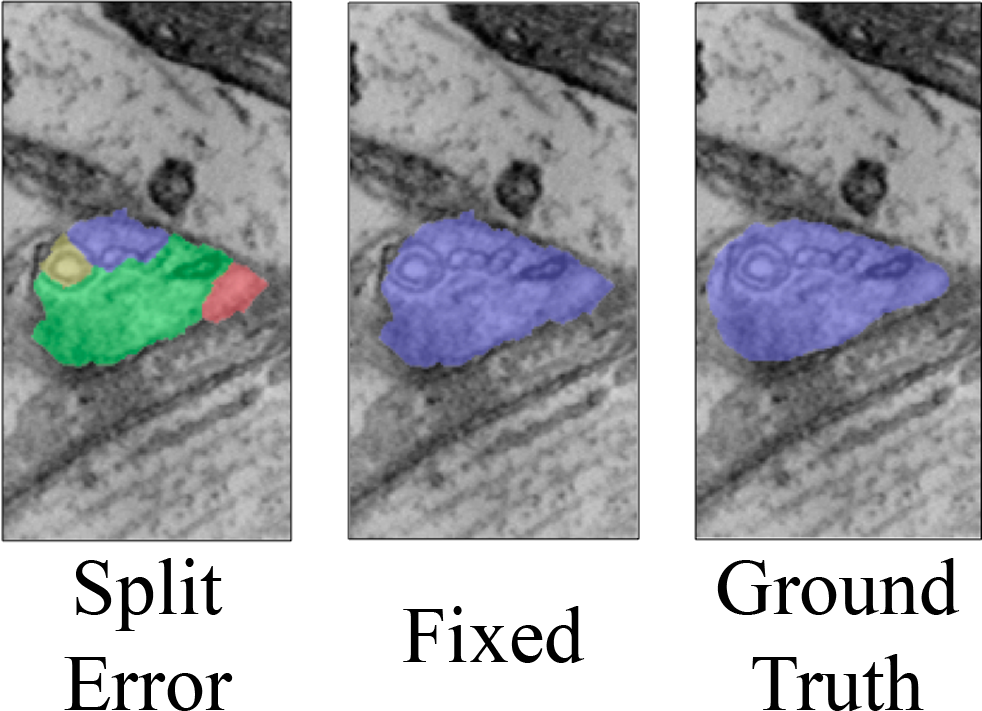
\includegraphics[width=.35\textwidth]{gfx/spliterror_2.png}
\qquad
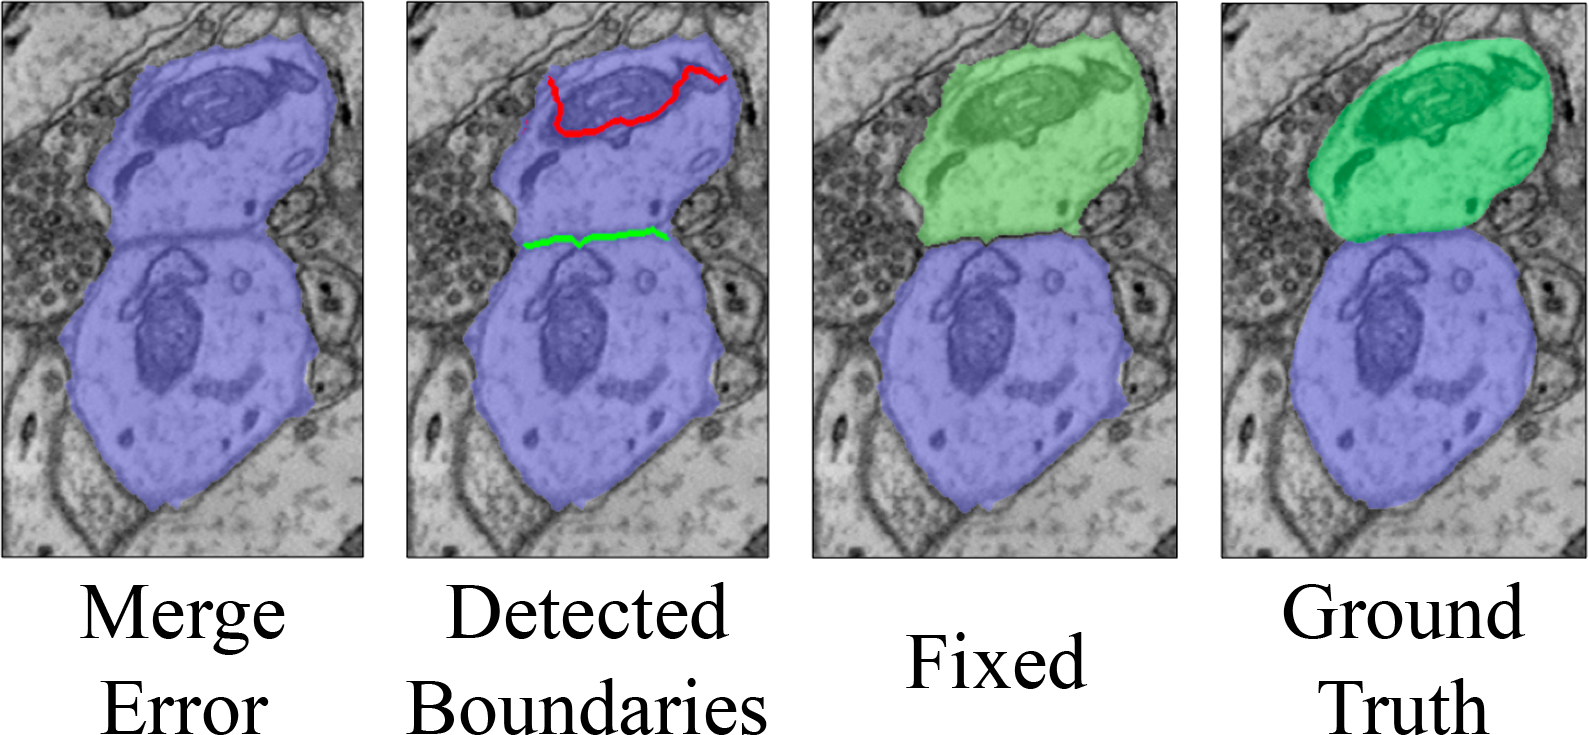
\includegraphics[width=.55\textwidth]{gfx/mergeerror.png}
\caption{Split and merge error examples, their corrections, and their ground truths.}
\label{fig:merge_error}
\end{figure}

%Paragraph three: What is the proposed solution at a high level? What is the result of the method, and how does it impact the problem?
Our goal is to add automatic detection of split and merge errors to proofreading tools. Instead of the user visually inspecting the whole data volume carefully to spot errors, we design automatic classifiers that detect split and merge errors in 2D segmentations. Then, a proofreading tool can recommend regions with a high probability of an error to the user, and suggest corrections to accept or reject. We call this process \textit{Guided Proofreading}.

The initial automatic segmentation is constrained by the data rate of the microscope. Given a membrane segmentation from a fast automatic method, our classifiers operate on whole cell regions, which relaxes the constraint on speed. Compared to techniques that must analyze every input pixel, this boundary assessment focus reduces the data analysis to the boundaries only and so allows us to employ wider convolutional neural networks that take regional context and multiple input channels into account. One reason to classify errors on 2D images lies with the cost of 3D registration. This is often slow as it requires non-linear image alignment \cite{akselrod09,Saalfeld2010Asrigidaspossible}. However, typically segmentation results are local decisions at the cell level. In this case, 3D reconstruction is unnecessary and, instead of waiting for the 3D output, proofreading can start immediately to maximize error correction before cell grouping occurs across sections.

%Paragraph five: Optimistically, what is the consequence of the method - what can I do now that I could not do before?
We quantitatively validate our approach with variation of information (VI) versus ground truth expert segmentations. While unintuitive, VI is a common metric to evaluate region segmentation performance \cite{NunezIglesias2013Machine}. We compare our approach in an experiment against an existing proofreading tool that provides only semi-automatic merge error correction~\cite{haehn_dojo_2014}. Here, with a simulated user, our automatic error suggestions and corrections decrease VI from 0.4764 to 0.3996, which is in contrast to pure manual or pure automatic methods that can both increase the VI. In addition, on a larger dataset, our method decreases VI from 0.4847 to 0.3946. As a consequence, we are able to provide tools to proofread segmentations more efficiently, and so better tackle large volumes of connectomics imagery.

%\subsection{Contributions}
%
%Given this, we contribute to the literature:
%\begin{enumerate}
%\item One contribution
%\item Two contribution
%\item (Maybe) three contribution
%\end{enumerate}
%
%\begin{figure}
%\missingfigure{Example of a fixed split error. Example of a fixed merge error.}
%\caption{Example of a fixed split error. Example of a fixed merge error.}
%\end{figure} % Now contains related work
\section{Related Work}

\paragraph{Automatic Segmentation}

Multi-terabyte EM brain volumes require automatic segmentation~\cite{jain2010,kaynig10,Liu2014,NunezIglesias2013Machine,GALA2014,amelio_segmentation}, but this data can be hard to classify in cases with ambiguous intercellular space. 

The 2013 IEEE ISBI neurites 3D segmentation challenge~\cite{isbi_challenge} showed that existing algorithms which learn from expert-segmented training data still exhibit high error rates. NeuroProof \cite{neuroproof2013} allows interactive learning of agglomeration of over-segmentations of images, based on a random forest classifier. Vazquez-Reina et al.~\cite{amelio_segmentation} propose automatic 3D segmentation by taking whole EM volumes into account rather than a per section approach, then solving a fusion problem with a global context. Kaynig et al.~\cite{kaynig10} propose a random forest classifier coupled with an anisotropic smoothing prior in a conditional random field framework and 3D segment fusion. 

It is also possible to learn segmentation classification features directly from images with CNNs. Ronneberger et al.~\cite{RonnebergerFB15} use a contracting/expanding CNN path architecture to enable precise boundary localization with small amounts of training data. Lee et al.~\cite{lee2015recursive} recursively train very deep networks with 2D and 3D filters to detect boundaries. 

While these approaches make good progress, in general proofreading is required to improve them through generating more ground-truth segmentations.

Arganda-Carreras et al.~\cite{10.3389/fnana.2015.00142} posed the ISBI 2D EM segmentation challenge in 2012, where a 30-image corpus of fly cell `in/out' labels was used to train boundary detection. However, mouse brain EM data is more difficult than the ISBI 2012 challenge, as it contains large intercellular space which is hard to classify. 

Bogovic et al.~\cite{BogovicHJ13} learn 3D features, and show even that unsupervised learning can produce better features than hand-designs. In this paper, we extend the features reported by Bogovic et al. but limit the classification to 2D images rather than 3D. One major reason for attempting to classify errors on 2D images is with the scale of the task. 3D reconstruction pipelines are often slow as they require non-linear image alignment or registration \cite{akselrod09,beyer13,Saalfeld2010Asrigidaspossible}. However, typically segmentation results are local decisions at the cell level. In this case, reconstruction is unnecessary and, instead of waiting for the 3D output, proofreading can start immediately to maximize throughput.

\paragraph{Collaborative Interactive Segmentation}

Recent works attack the problem of massive volume segmentation through crowd-sourcing\cite{saalfeld09,anderson2011}. EyeWire~\cite{eyewire2012} asks novice users to participate in a segmentation game for segmenting neuronal structures using a semi-automatic algorithm. D2P ~\cite{Giuly2013DP2} uses a micro-labor workforce approach where local boolean decisions are combined to produce a consensus segmentation. In general, our goal is to correct the output of a segmentation which is thought to be good; hence, our tool would be used after learning a segmentation model to direct user attention to correct likely erroneous areas.

\paragraph{Proofreading Tools}
The bottleneck of editing an existing and imperfect automatic segmentation was identified by Peng et al. \cite{proofreading_bottleneck}. The authors developed software which supports three-dimensional proofreading. Also for 3D, Sicat et al. proposed a graph abstraction method to guide users to problematic regions indicating the need for corrections \cite{markus_proofreading}. Janelia Farms then introduced Raveler \cite{raveler}, a software targeting expert users by offering many parameters for tweaking the proofreading process at the cost of a higher complexity. Raveler also includes a simple 3D renderer to validate corrections across slices.

In 2014, Haehn et al. developed two proofreading tools: Mojo and Dojo. Mojo is a stand-alone proofreading tool with a simple scribble interface for error correction. The need for distributed proofreading lead us to develop Dojo, a web-based proofreading framework with a minimalistic user interface. The authors defined requirements for proofreading tools in general and then evaluated the accuracy and speed of Raveler, Mojo and Dojo through a quantitative user study (Sec. 3 and 4) \cite{haehn_dojo_2014}. 
Al-Awami et al. then integrated Dojo into their proofreading management system Neuroblocks \cite{Neuroblocks}. The system includes a scalable visualization for tracking the proofreading process among multiple users.

In 2015, Karimov et al. proposed a guided volume editing approach using histogram dissimilarity \cite{karimov_guided_volume_editing}. Measuring differences in histogram distributions helps their system to find potential errors and to suggest possible corrections. Their method shows promising results on Computed-Tomography Angiography datasets but is targeted towards expert users.

Recently, Uzunbas et al. showed that potential labeling errors can be found by taking the merge tree of an automatic segmentation method into account \cite{uzunbas}. The authors keep track of uncertainties during the automatic labeling and then present them as regions for proofreading. This requires access to the merge tree of the segmentation stage which is not always available.


%\subsection{Contributions}

%Given this, we contribute to the literature:
%\begin{enumerate}
%\item One contribution
%\item Two contribution
%\item (Maybe) three contribution
%\end{enumerate}
\begin{figure}[t]
 \centering
    \subfloat[CNN Layers\label{fig:layers}]{%
      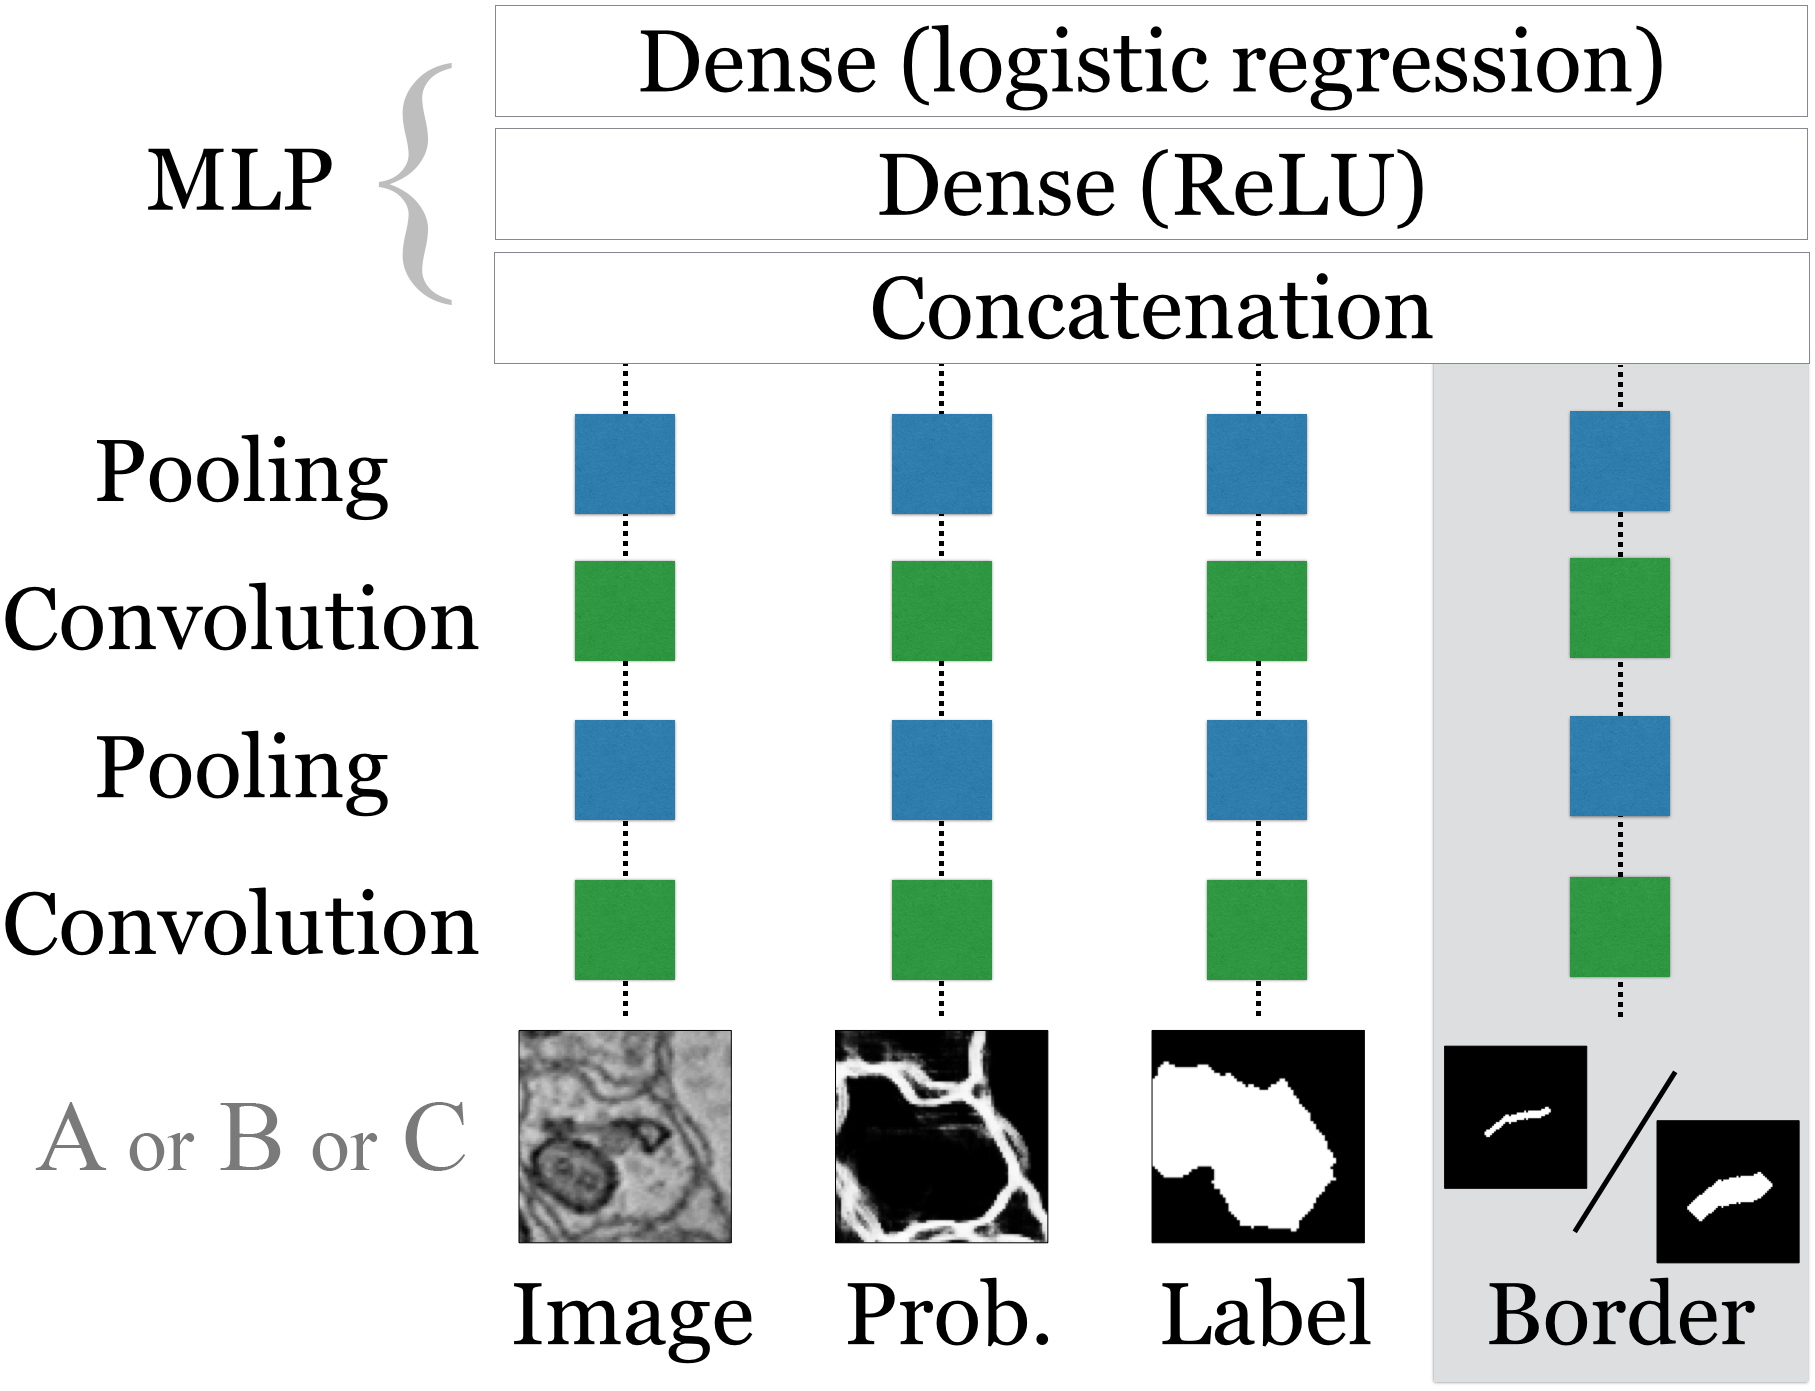
\includegraphics[width=0.9\textwidth]{gfx/network.png}
    }

    \subfloat[Network configurations\label{fig:networks}]{%
      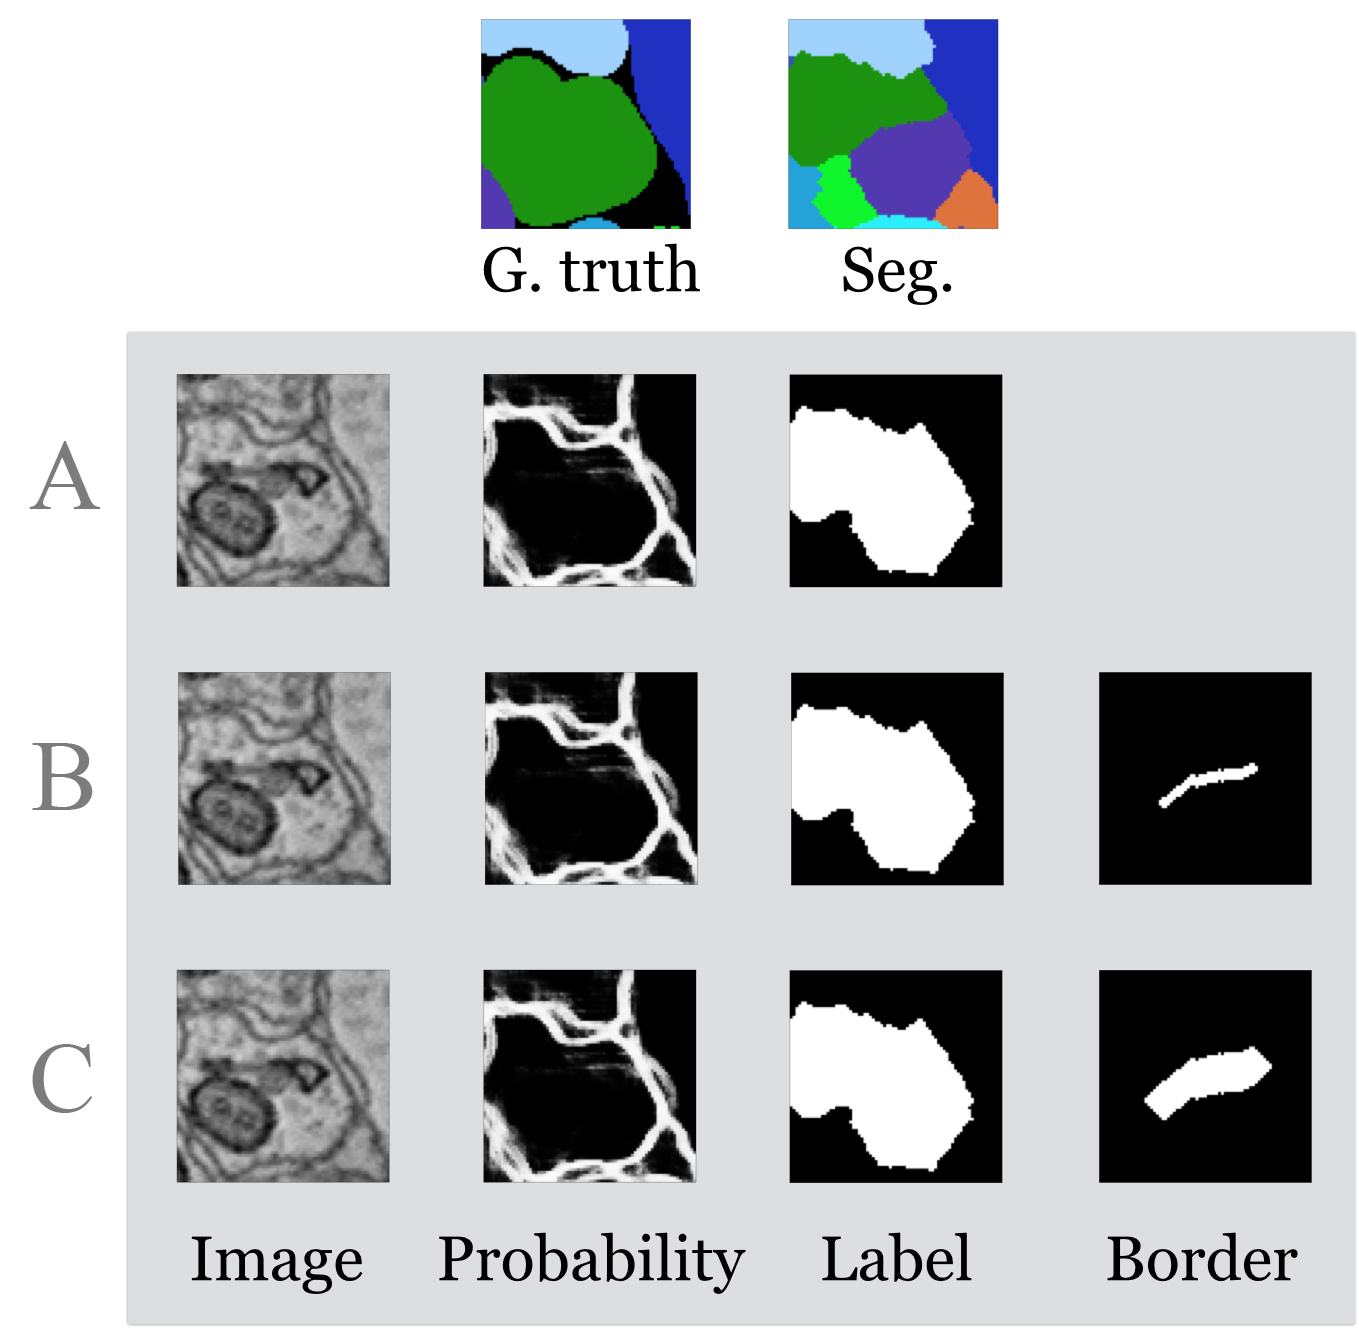
\includegraphics[width=0.9\textwidth]{gfx/network_inputs.png}
    }
	\caption{(a) Our network architecture with up to four input channels, each with two convolutional and two pooling layers. MergeNet includes four separate input channels and RGBANet uses a 4-channel input. (b) We trained three different network configurations with three and four inputs: A) image, boundary map probability, and merged binary mask; B) A configuration extended with a small border mask, to focus on the specific boundary in question; C) A configuration extended with a large border mask.}

\end{figure}


\begin{figure*}[ht]
%\ffigbox[][\textwidth]{
\begin{floatrow}

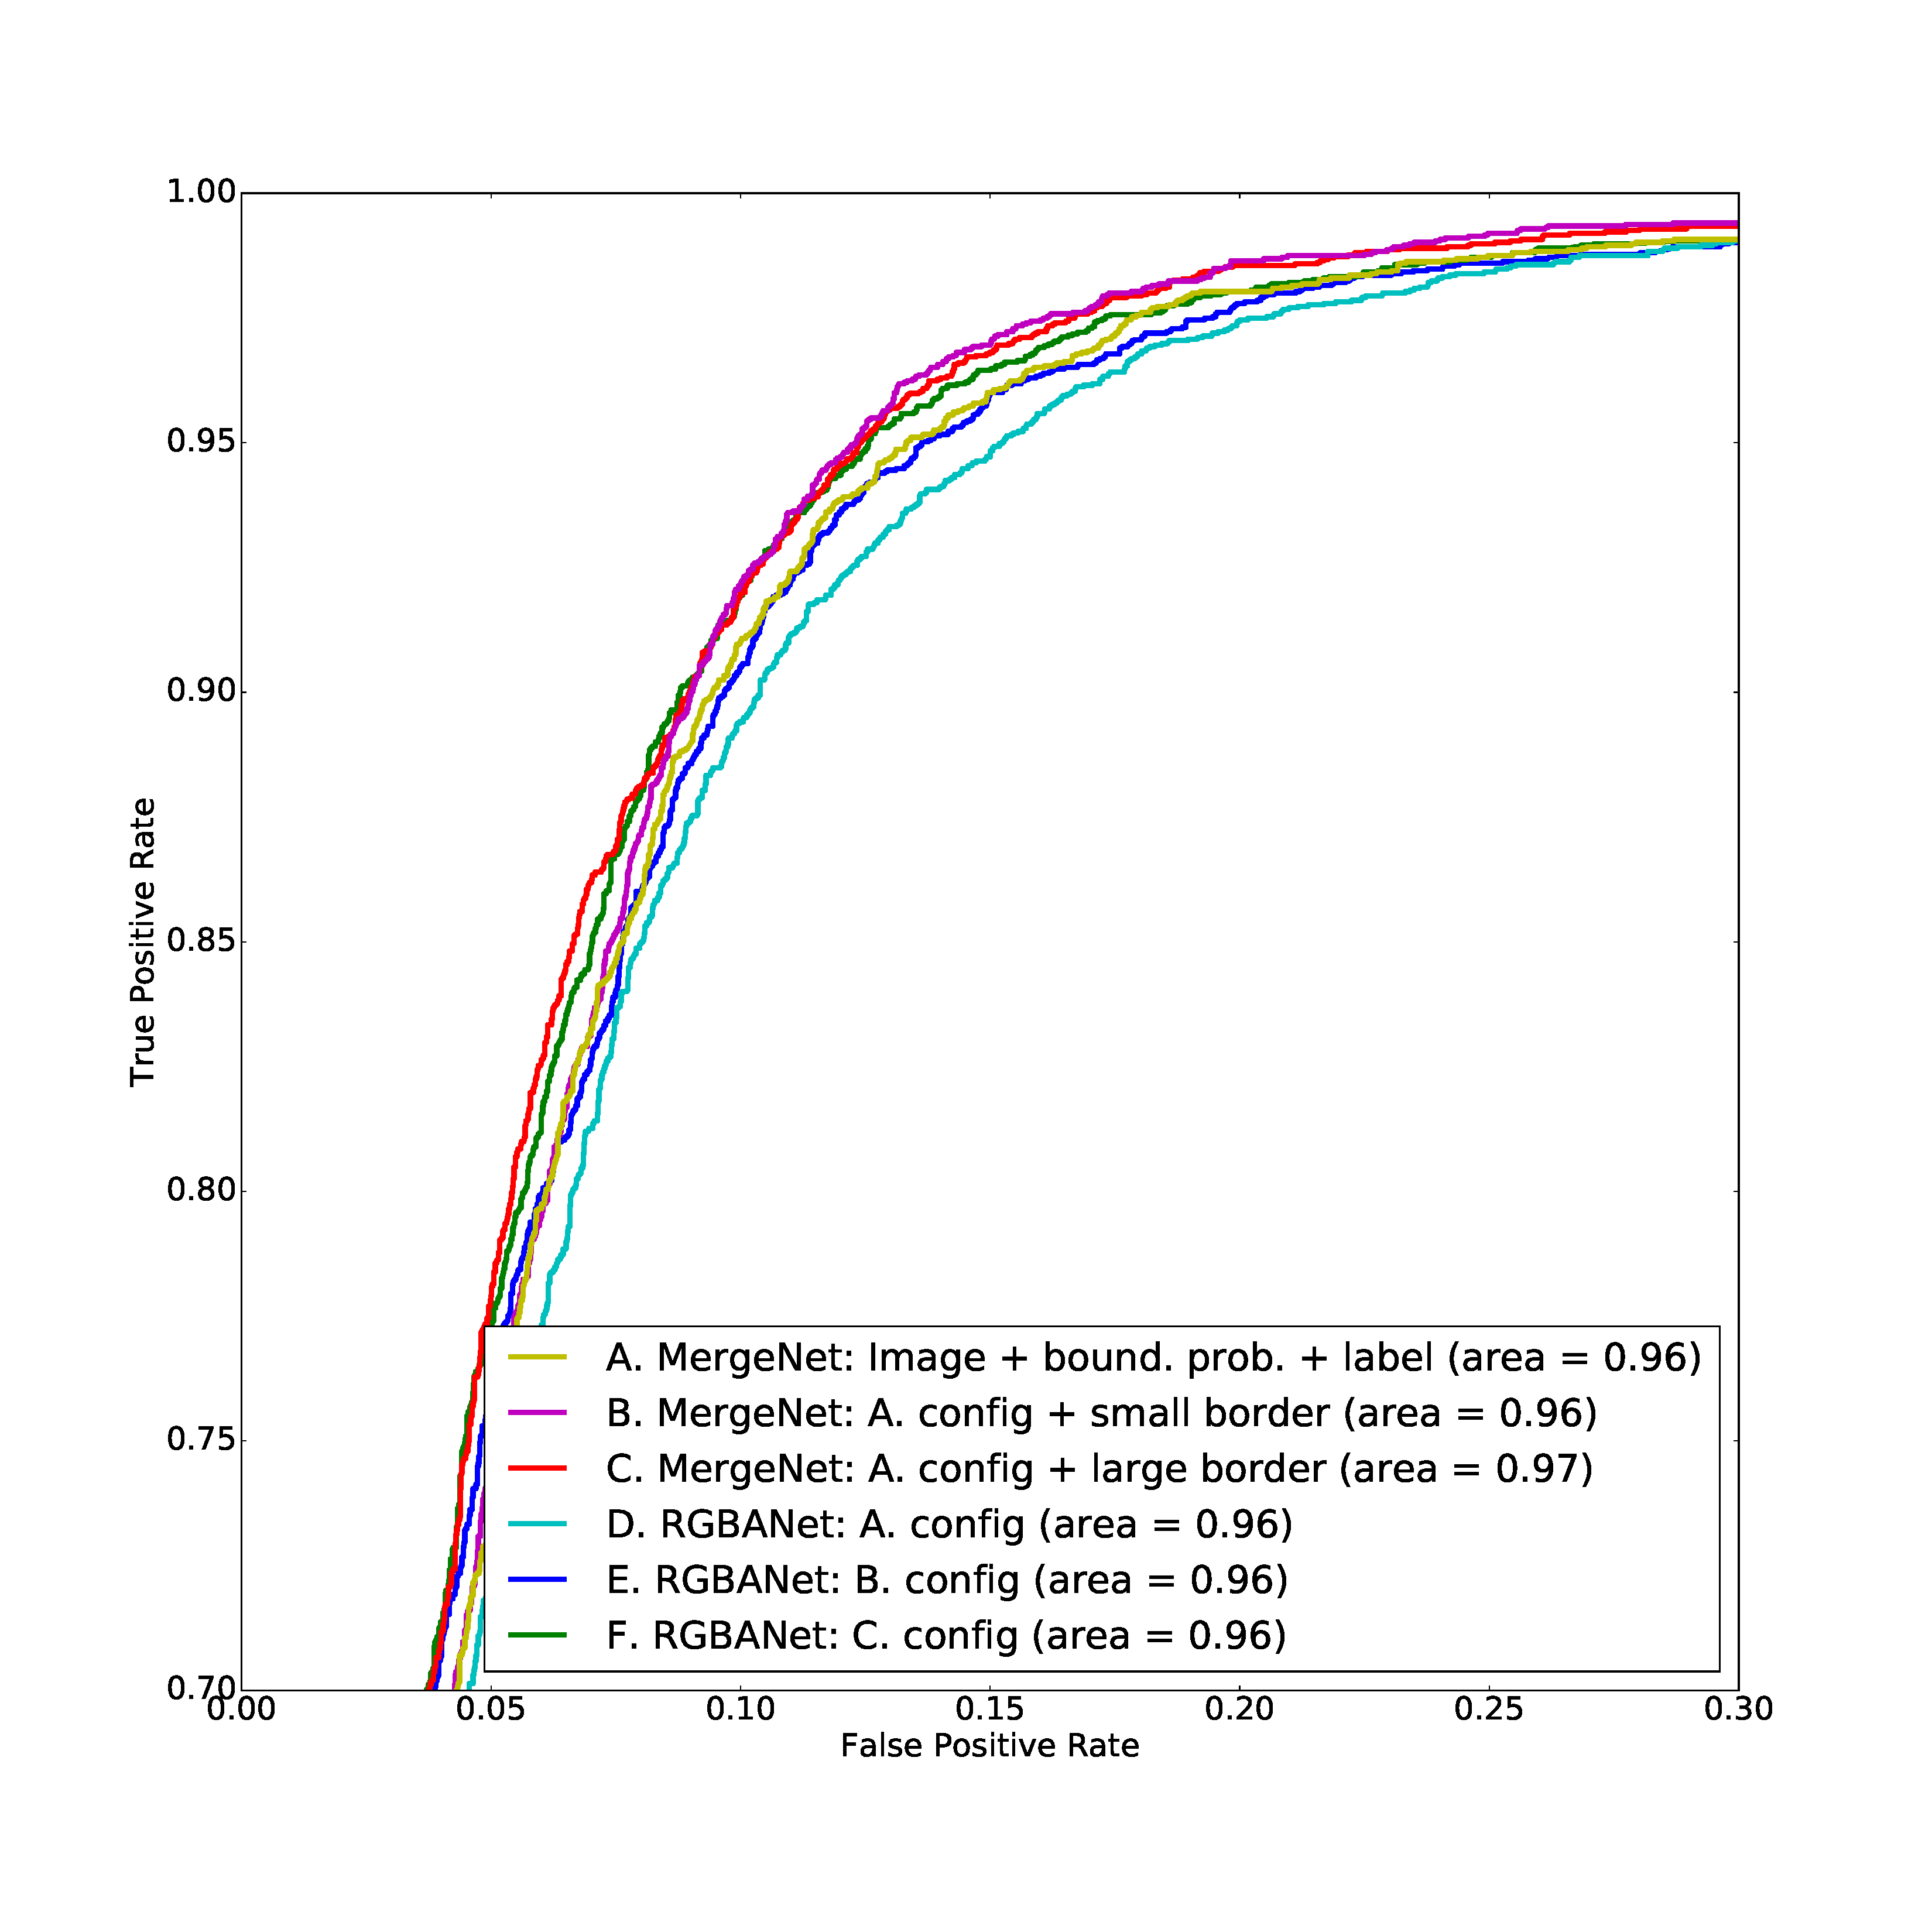
\includegraphics[width=.5\textwidth]{gfx/roc_plot.pdf}
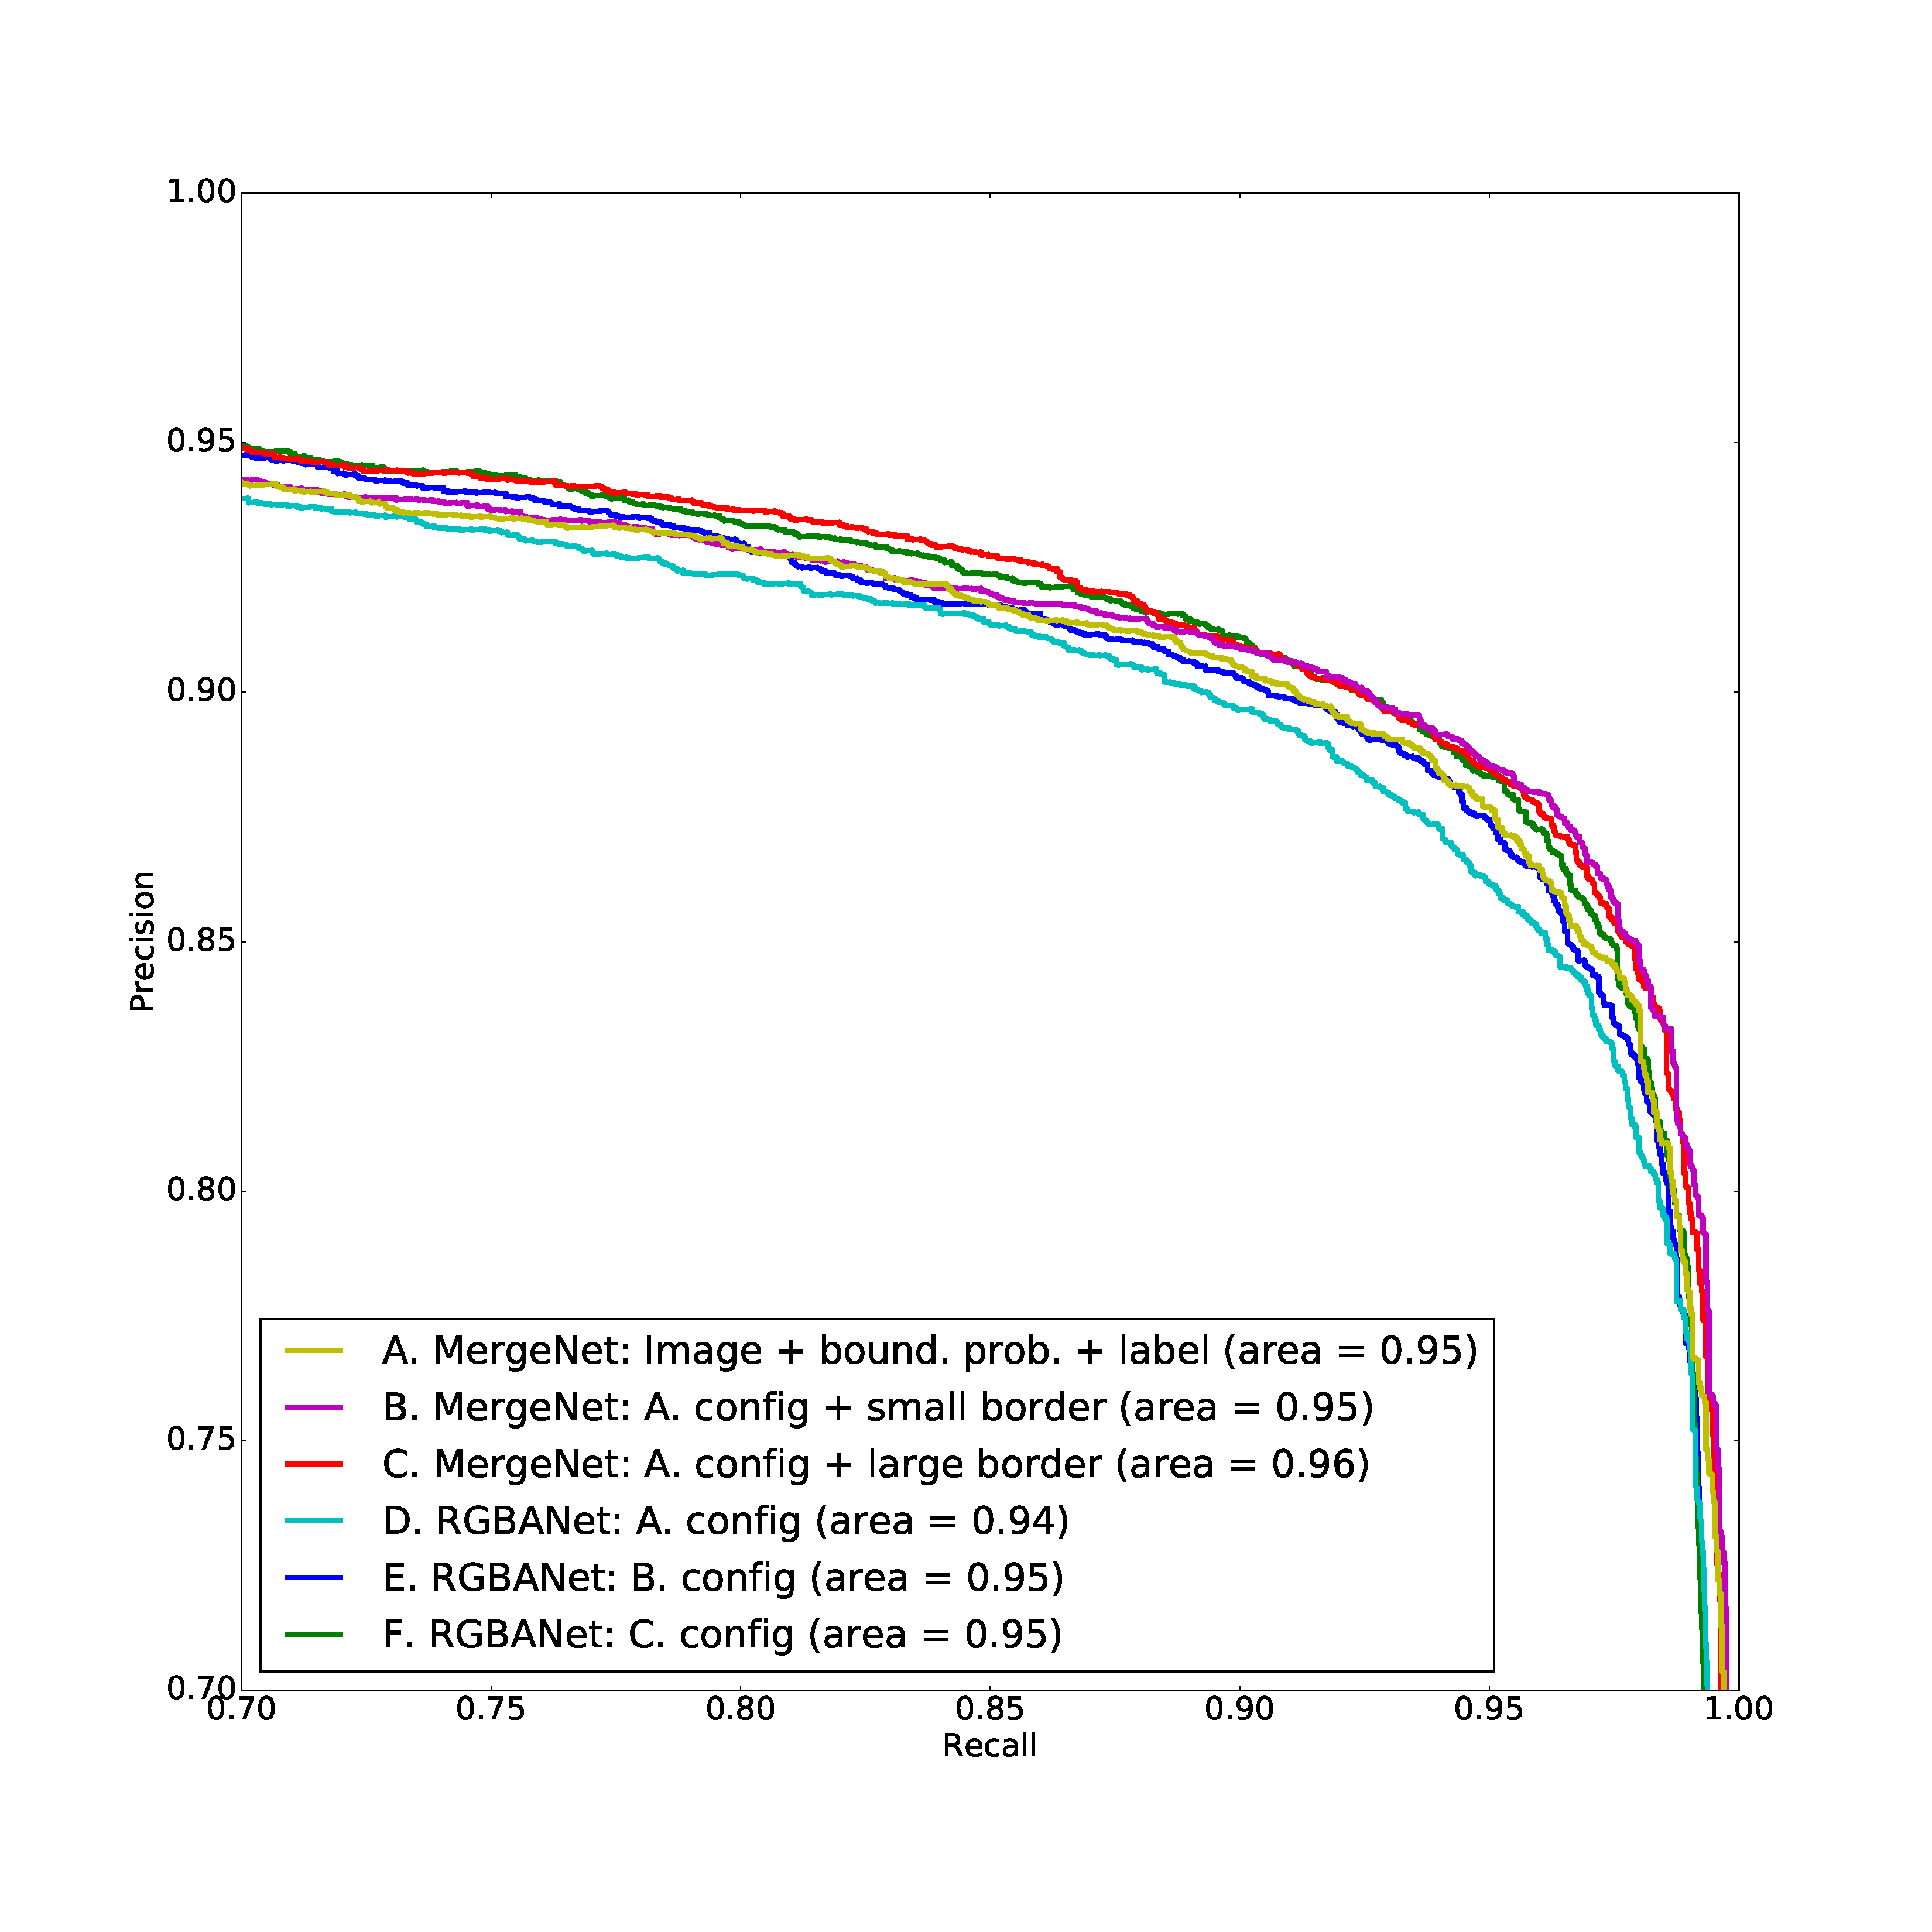
\includegraphics[width=.5\textwidth]{gfx/pr_plot.pdf}
\end{floatrow}

\begin{tabular}{l rrrr}
\toprule
Network & Validation loss & Test acc. ~(\%) & Prec./Recall & \hspace{0.1cm} F1 Score \\
\midrule
A. MergeNet: Image + boundary prob. + seg. label & 0.073 & 0.906 & 0.906/0.906 & 0.907 \\
B. MergeNet: A config. + small border overlap ($d=1$) & 0.07 & 0.911 & 0.911/0.911 & 0.912 \\
C. MergeNet: A config. + large border overlap ($d=5$) & 0.07 & 0.908 & 0.908/0.908 & 0.909 \\
D. RGBANet: A. config. & 0.058 & 0.895 & 0.895/0.895 & 0.894 \\
E. RGBANet: B. config. & 0.054 & 0.907 & 0.907/0.907 & 0.908 \\
F. RGBANet: C. config. & 0.058 & 0.905 & 0.905/0.905 & 0.904\\
%A. Image + boundary prob. + seg. label & 0.3853 & 0.4163 & 81.15 \\
%B. A config. + small border overlap($d=1$) & 0.3798 & 0.3843 & 82.34\\
%C. A config. + large border overlap ($d=5$) &  0.3703 & 0.3919 & 83.02\\
%Bogovic et al. + small border overlap($d=1$) & 0.379833 & 0.384347 & 82.34\\
%Bogovic et al. + large border overlap ($d=5$) &  0.370280 & 0.391911 & 83.02\\
\bottomrule
\end{tabular}

%\end{floatrow}
%}{
 \caption{Network design training evaluation. Adding an extra channel containing a binary mask of just the border slightly increases performance in both network configurations. Due to slightly larger areas under the curves for both receiver operating characteristic and precision/recall, we choose configuration MergeNet C to evaluate VI against human performance.}
 \label{fig:trainingperformance}
%}
\end{figure*}


\begin{figure*}[t]
 \centering
    \subfloat[Interactive (Dojo) vs. Guided Proofreading\label{fig:dojo_vi}]{%
		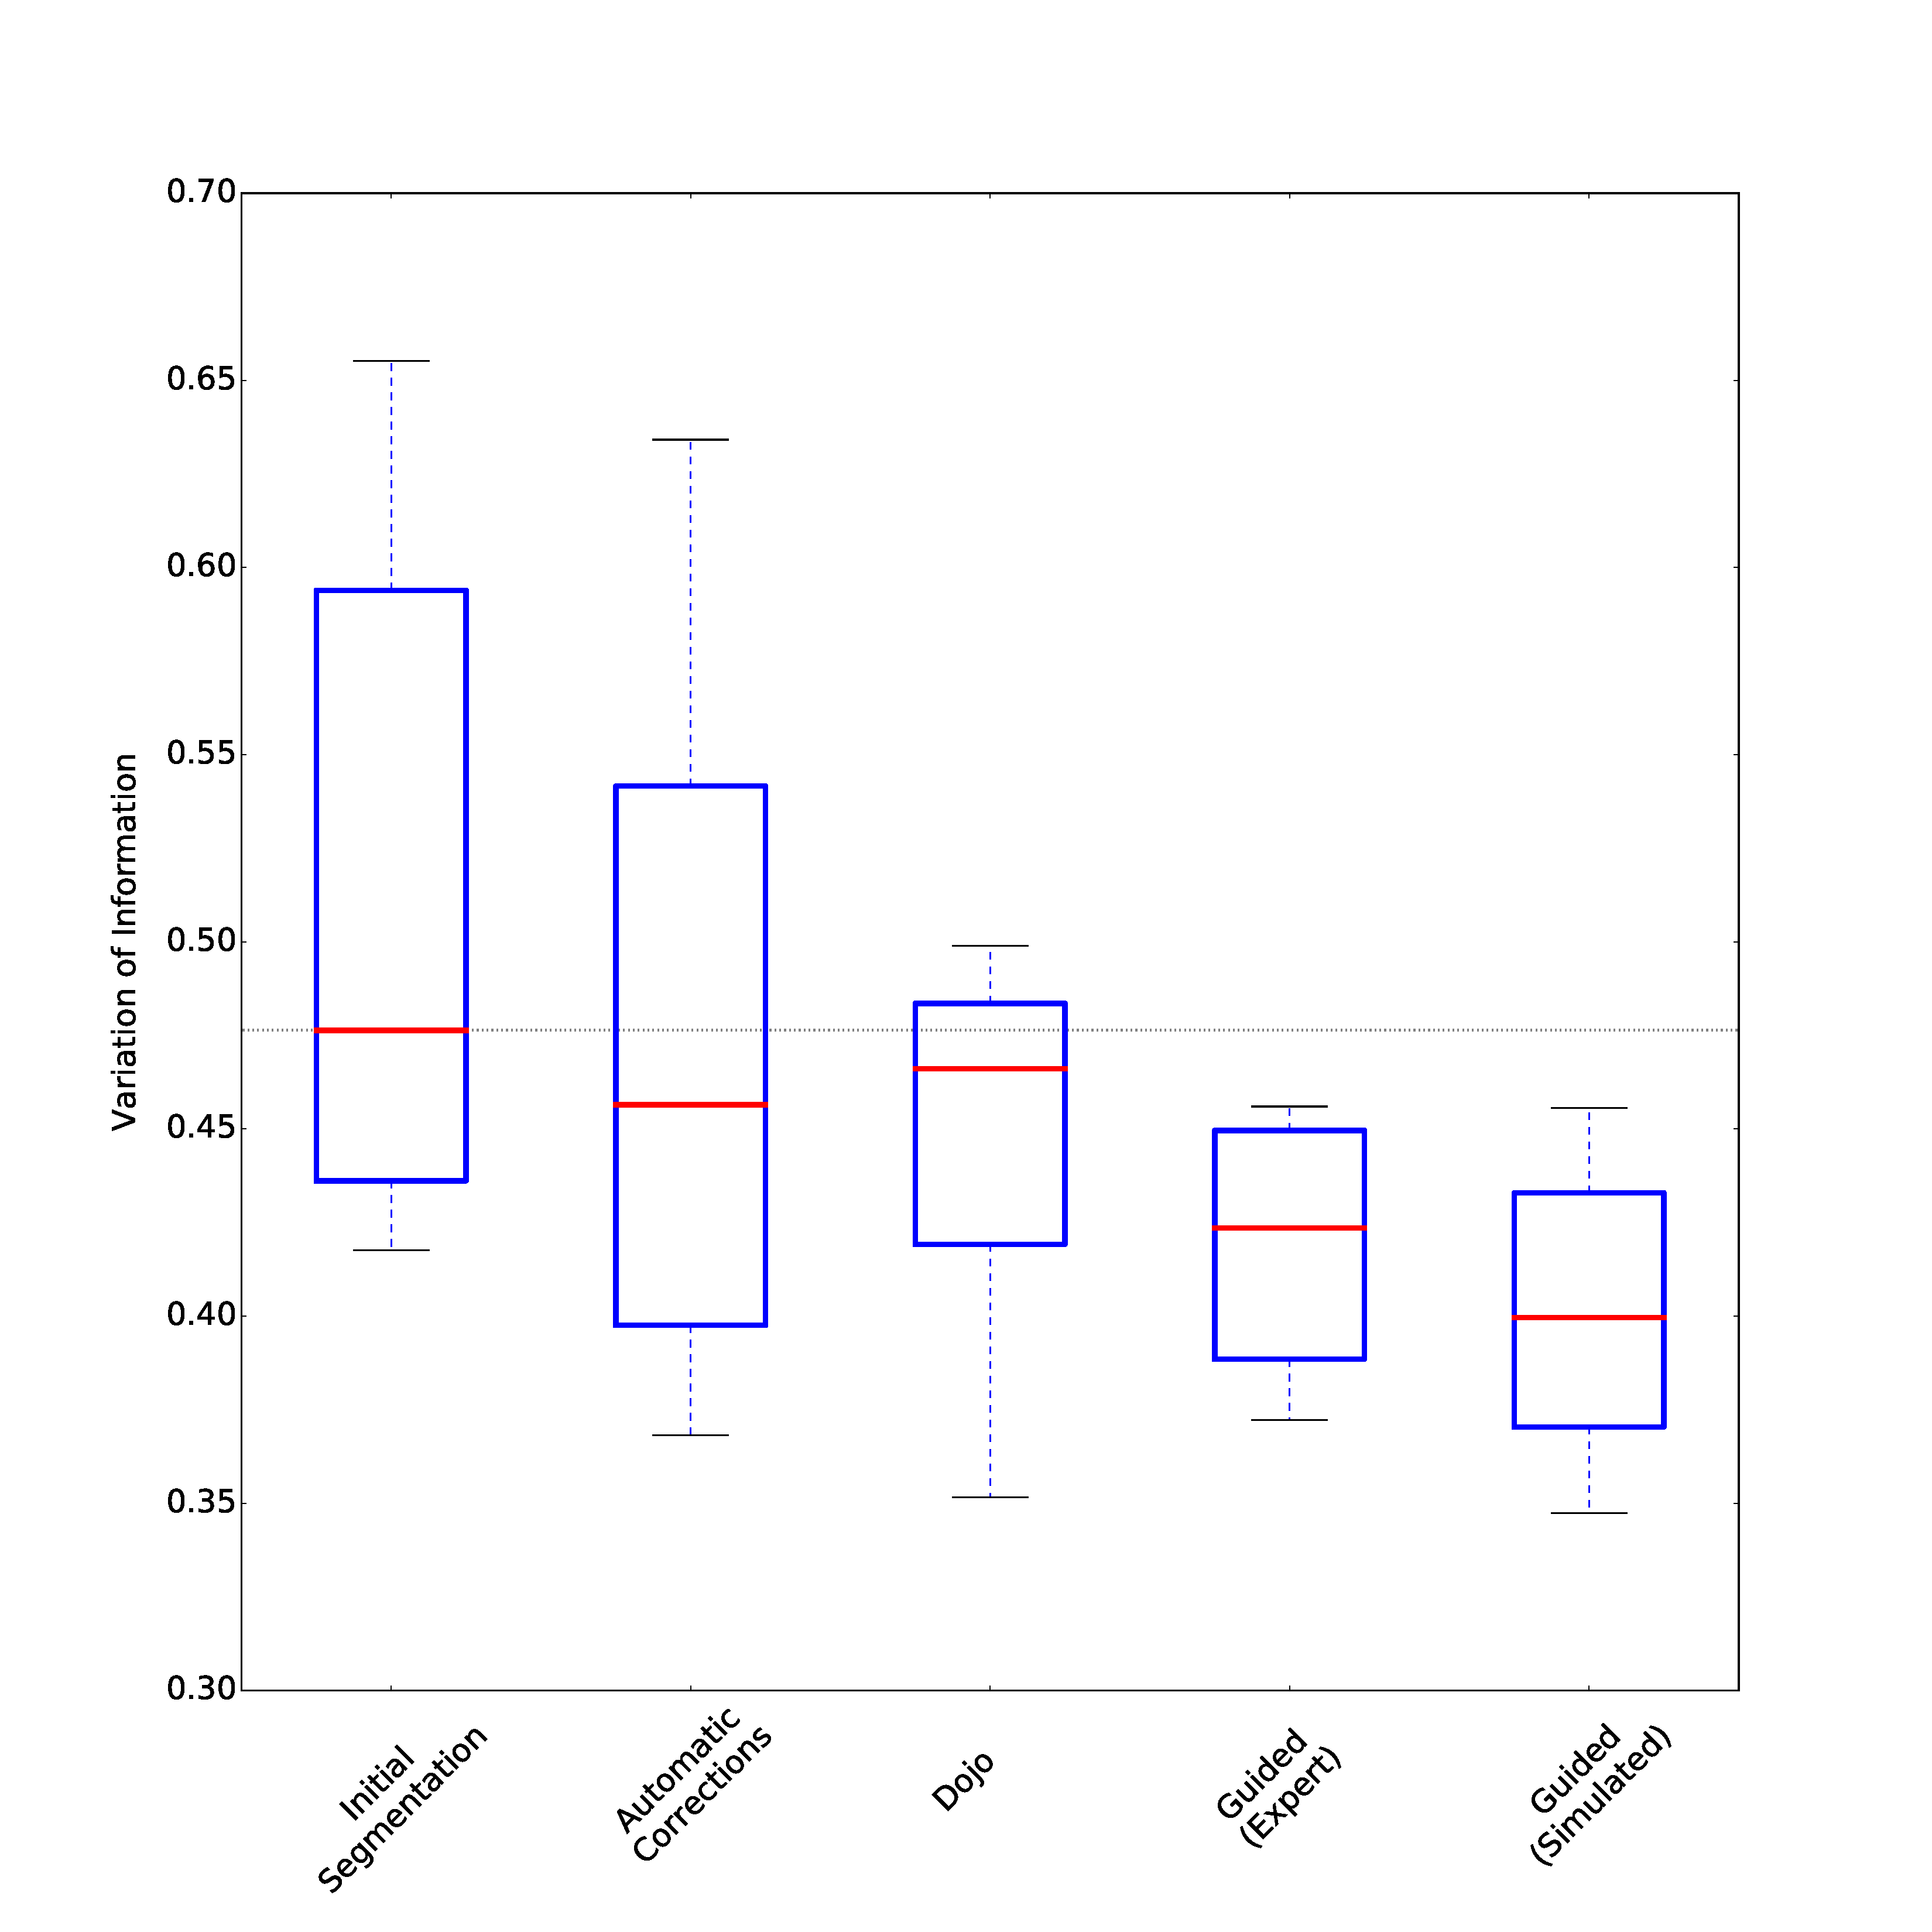
\includegraphics[width=.45\textwidth]{gfx/dojo_vi.pdf}
    }
    \hfill
    \subfloat[Simulated User Error Rate\label{fig:dojo_error_rate}]{%
	    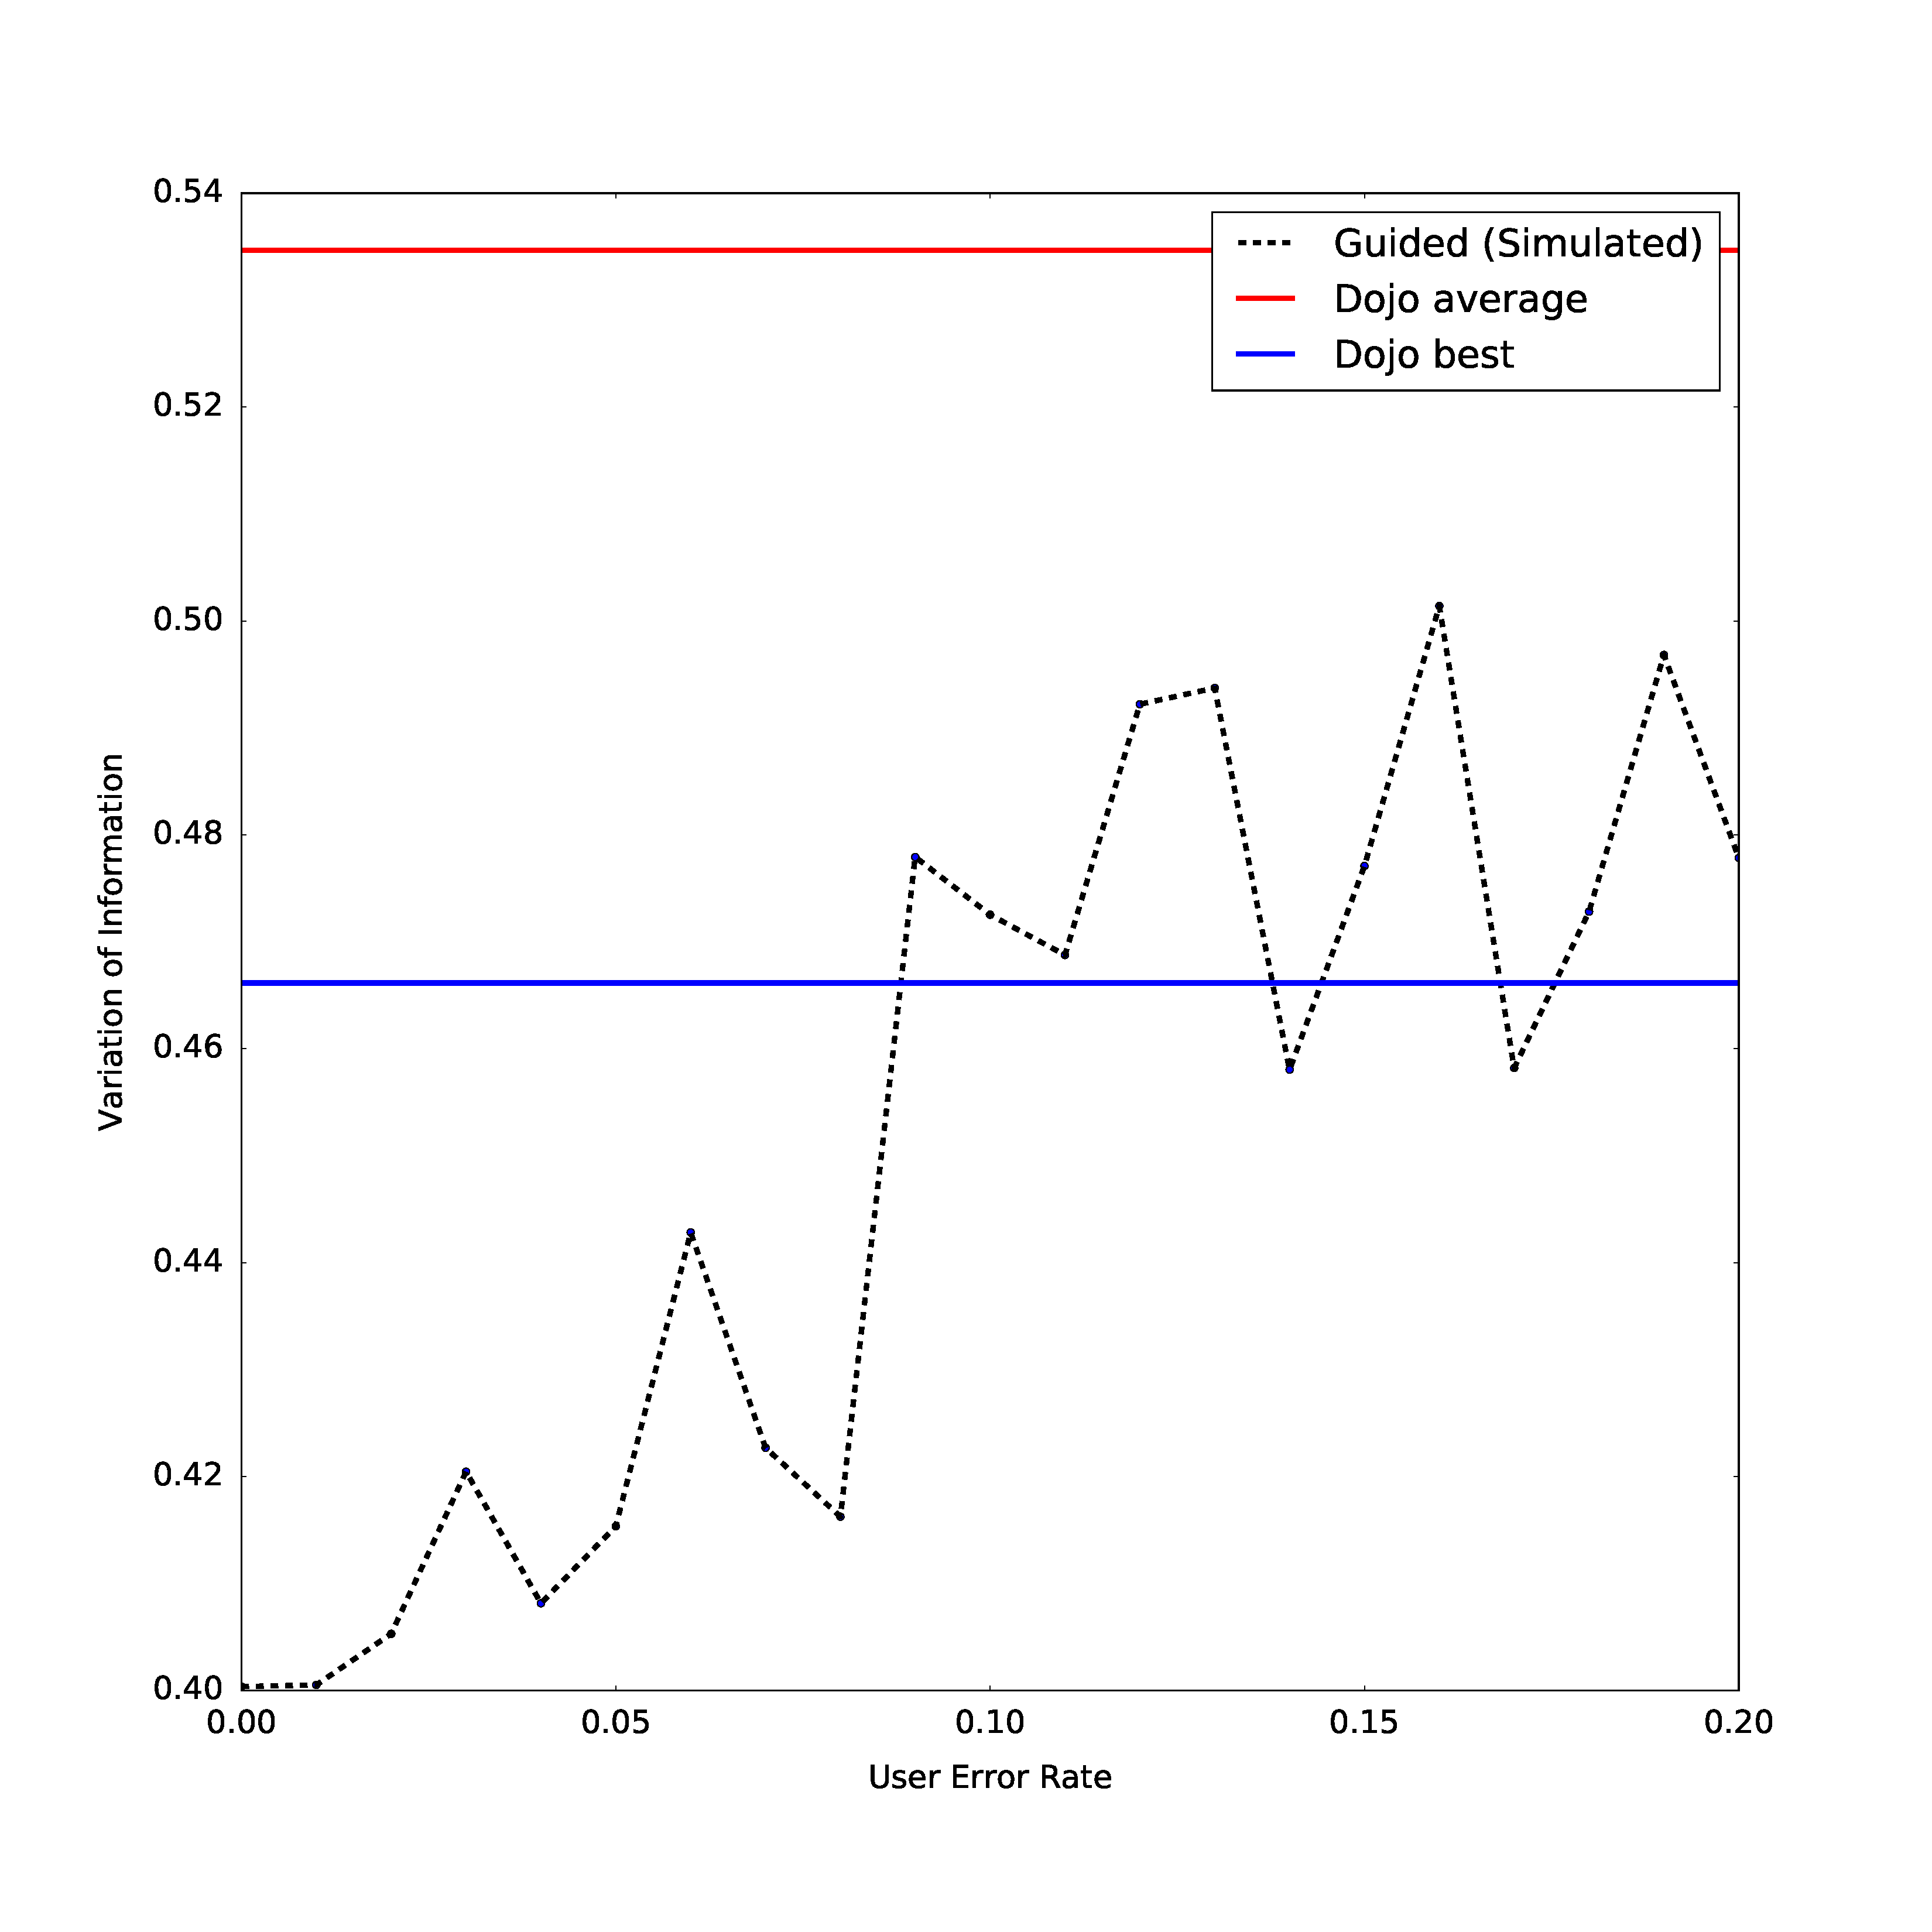
\includegraphics[width=.45\textwidth]{gfx/dojo_errorrate.pdf}
    }

\caption{(a) We compare distributions of VI measures across 10 sections for the initial automatic segmentation, a fully-automatic correction of recommended errors based on a threshold of acceptance, the best user in the Haehn et al.~experiment with Dojo, two experts using our system and our simulated user. Lower scores are better. (b) We test our simulated user with different error rates and compared against the best user as well as the average user performance in Dojo.}
\label{fig:results}

\end{figure*}


\section{Method}
%Paragraph one: Overview of the method. What are the high level steps taken to build the system? What are the key techniques used within the system?
We build a split error classifier using a convolutional neural network (CNN) to check the boundaries of an existing automatic segmentation. For each boundary, the CNN provides a probability that points sampled along the boundary have caused a split error. For each boundary, we sample up to 10 decision points, where the decision points are spread evenly over the boundary length, given that their context windows do not overlap. These probabilities are then weighted by the length of the boundary within the context over the total boundary length, and averaged. A greedy algorithm then merges neighboring regions sequentially, starting with the highest probability score. Following each merge, neighboring boundaries are re-evaluated for split errors. Correcting a split error is as simple as merging the two bordering labels.

Identification and correction of merge errors is more challenging, because we must look inside segmentation regions for missing or incomplete boundaries and then propose the correct boundary. However, we can reuse the same trained CNN for this task. For each segmentation label, we generate 30 potential boundaries through the region by placing watershed seed points at opposite sides of the label boundary and generating the corresponding split. Then, we check to see whether any potential edge is classified as a split error. If the CNN detects a boundary with a very low split error score, then the boundary should have been in the segmentation and the region is a candidate for a merge error.
%\JT{Candidate for figure - this potential boundary generation is a bit tricky to follow.}\VKF{Maybe put some more candidates into Figure 1 as examples?}



%\begin{figure}[t]
%\centering
%\includegraphics[scale=.15]{gfx/patches.pdf}
%\caption{\JT{NEW CAPTION PLEASE.}}
%\label{fig:patches}
%\end{figure}




\subsection{Convolutional Neural Network Design}
%Paragraph: What is the rationale behind our network design? Why do we think this will work over other approaches?
To train a CNN for split error detection we take multiple channels of context information of the boundary into consideration for the decision making process. We pass multiple inputs into the CNN windowed around a particular decision point or pixel: the input grayscale image patch, the corresponding boundary probability map patch, and two corresponding binary mask patches for the segmented regions at either side of the boundary. Following Bogovic et al.~\cite{BogovicHJ13}, these two masks can be combined into a single mask with comparable performance (configuration A, Fig.~\ref{fig:networks}). The network then leverages these multiple input patches to identify and correct errors made by the previous membrane detection network and automatic segmentation pipeline.

One way to combine these inputs is to treat them as a 4-channel input, so that alignment between the input image and the segmentation masks are not lost throughout the convolutions. We refer to this approach as \textit{RGBANet}. However, training a boundary-classifying network can be difficult due to rigid ground-truth segmentations, which often differ substantially from automatic segmentation regions in ambiguous extra-cellular space. To cope with this variation, our network is based on multiple separate input channels (Fig.~\ref{fig:layers}). Each of the input patches is connected individually to a 2-layer network, with each layer consisting of convolutional and pooling layers. The output of these networks is then combined by a fully connected multi-layer perceptron (MLP) with one hidden layer and a two class logistic regression output layer. The intuition for this multiple input channel approach is that we want to allow variation in the input and masks independently, to accommodate potential error, and then for the hidden layers to discover appropriate combinations of the relevant features learned separately for the different input channels. We refer to this approach as \textit{MergeNet}.

To better direct both networks to train on the true boundary edge, which in many cases is missing from the boundary probability map and hence is the cause of merge errors, we additionally pass as input a second binary mask. This mask contains the true boundary edge (configuration B, Fig.~\ref{fig:networks}). To consider slight edge ambiguities, we also test a version of this network where the true boundary mask has been dilated by 5 pixels (configuration C).



\subsection{Training}
To train the network, we use the blue 3-cylinder mouse cortex volume of Kasthuri et al. \cite{kasthuri2015saturated} ($2048\times2048\times300$ voxels). The tissue is dense mammalian neuropil from layers 4 and 5 of the S1 primary somatosensory cortex of a healthy mouse. The resolution of our dataset is $3\, nm$ per pixel, and the section thickness is $30\, nm$. 
%\VKF{For the initial automatic segmentation, we train an existing pipeline on a similar dataset}. 
A manually-labeled expert segmentation is available as a ground truth for the entire dataset. We use the first 250 sections of the data for training and validation (split 0.25) and the last 50 for testing. To generate training data, we identify correct regions and split errors in the automatic segmentation by intersecting with the ground truth regions. From these regions, we sample 266,088 correct regions and 266,088 split error patches. As patch size, we defined $75\times75$ pixels to cover approximately $80\%$ of all boundaries in our segmentation output. 
%#   Training data:
%#   Patch size: (75,75)
%#   79828 correct splits
%#   79828 split errors
%#   rotated 90,180,270 degrees after each epoch
%
%#   validation data: 7464 correct splits + 7464 split errors
%#   test data: 5748 correct splits + 5748 split errors



We train our networks using the following parameters: learning rate $lr=0.03$ (iteratively decreasing until $lr=0.00001$), momentum $m=0.9$ (iteratively increasing until $m=0.999$), filter size $fs=13\times13$ and number of filters $fn=16$ for MergeNet ($fn_1=64, fn_2=48$ for RGBANet). This results in approximately 1.5 million parameters for all network configurations. For regularization we use dropout layers after each pooling layer with $p=0.2$. We assume that the training has converged if the validation loss does not decrease for 50 epochs. The network is specified using the deep learning libraries Lasagne and Theano \cite{Bastien-Theano-2012}, and trained on a Tesla K40m graphics card.

Figure \ref{fig:trainingperformance} presents validation loss function scores (cross validation), test accuracy percentages, precision/recall scores, and F1 scores. We also show receiver operating characteristics and precision/recall curves. Based on these performances and due to slightly larger area under the curves, we select configuration MergeNet C to evaluate against human performance in a VI improvement experiment. 







%\subsection{Error Discovery and Correction}

%\VKF{Our experiments have shown that the best average probability threshold to stop this process is in the range ($p_t=.7-1.0$) not sure what to do with this, I think this is from the test data? Do we need this still? At the moment it sounds weird}.
%\subsection{Merge Error Discovery and Correction}

%With the intuition that merge errors are caused by the failure to correctly detect a boundary, we can use the inverse probability of the split error classifier to help discover merge errors. For each segmentation region, we generate 30 possible splits across the region using watersheds seeded from the region boundary (Fig.~\ref{fig:merge_error}). Then, each candidate split is tested using our split error classifier. If the candidate split is 

%\VKF{Do we need this? If it stays we should not just hope. I think it can go if we publish the code. Further, we dilate the region segmentation by a fixed amount ($d=20$) prior to running watershed, hoping that one of the generated split edges clings to the boundary of the cell and then follows the correct splitting edge. To remove pixels that then overlap the boundary of the cell, we perform erosion by a fixed amount ($e=5$).} 

%
%\begin{table}
%\begin{tabular}{ll}
%\toprule
%Parameter & Value \\
%\midrule
%one & \\
%two & \\
%three & \\
%\bottomrule
%\end{tabular}
%\caption{This is a table of parameters. This is not very interesting, but it's easier to read than in the body text and putting everything together helps the reader quickly assess.}
%\end{table}
\section{Evaluation}
\label{sec:evaluation}
We evaluate our split and merge error detection and correction recommendation in the context of interactive proofreading tools: to direct users to regions with a high probability of error and to suggest corrections (Fig.~\ref{fig:results}). For comparison, we take publicly available mouse cortex data of the same kind as our training data. This data is part of the ISBI 2013 challenge training dataset ($1024\times1024\times100$ voxels) which was acquired using a serial section scanning electron microscope (ssSEM) with a resolution of $6\times6\times30\, nm$ per voxel. We use the available manually-labeled ground truth to score our approach using the variation of information (VI) metric, which is closely related to mutual information. VI is a measure of the distance between two clusterings, where lower VI numbers are better. Since our classifiers are trained on 2D image slices, we perform all evaluations on slices rather than 3D volumes.

\begin{figure}[t]
\centering
	%\subfloat[Segmentation test cases\label{fig:results}]{%
%	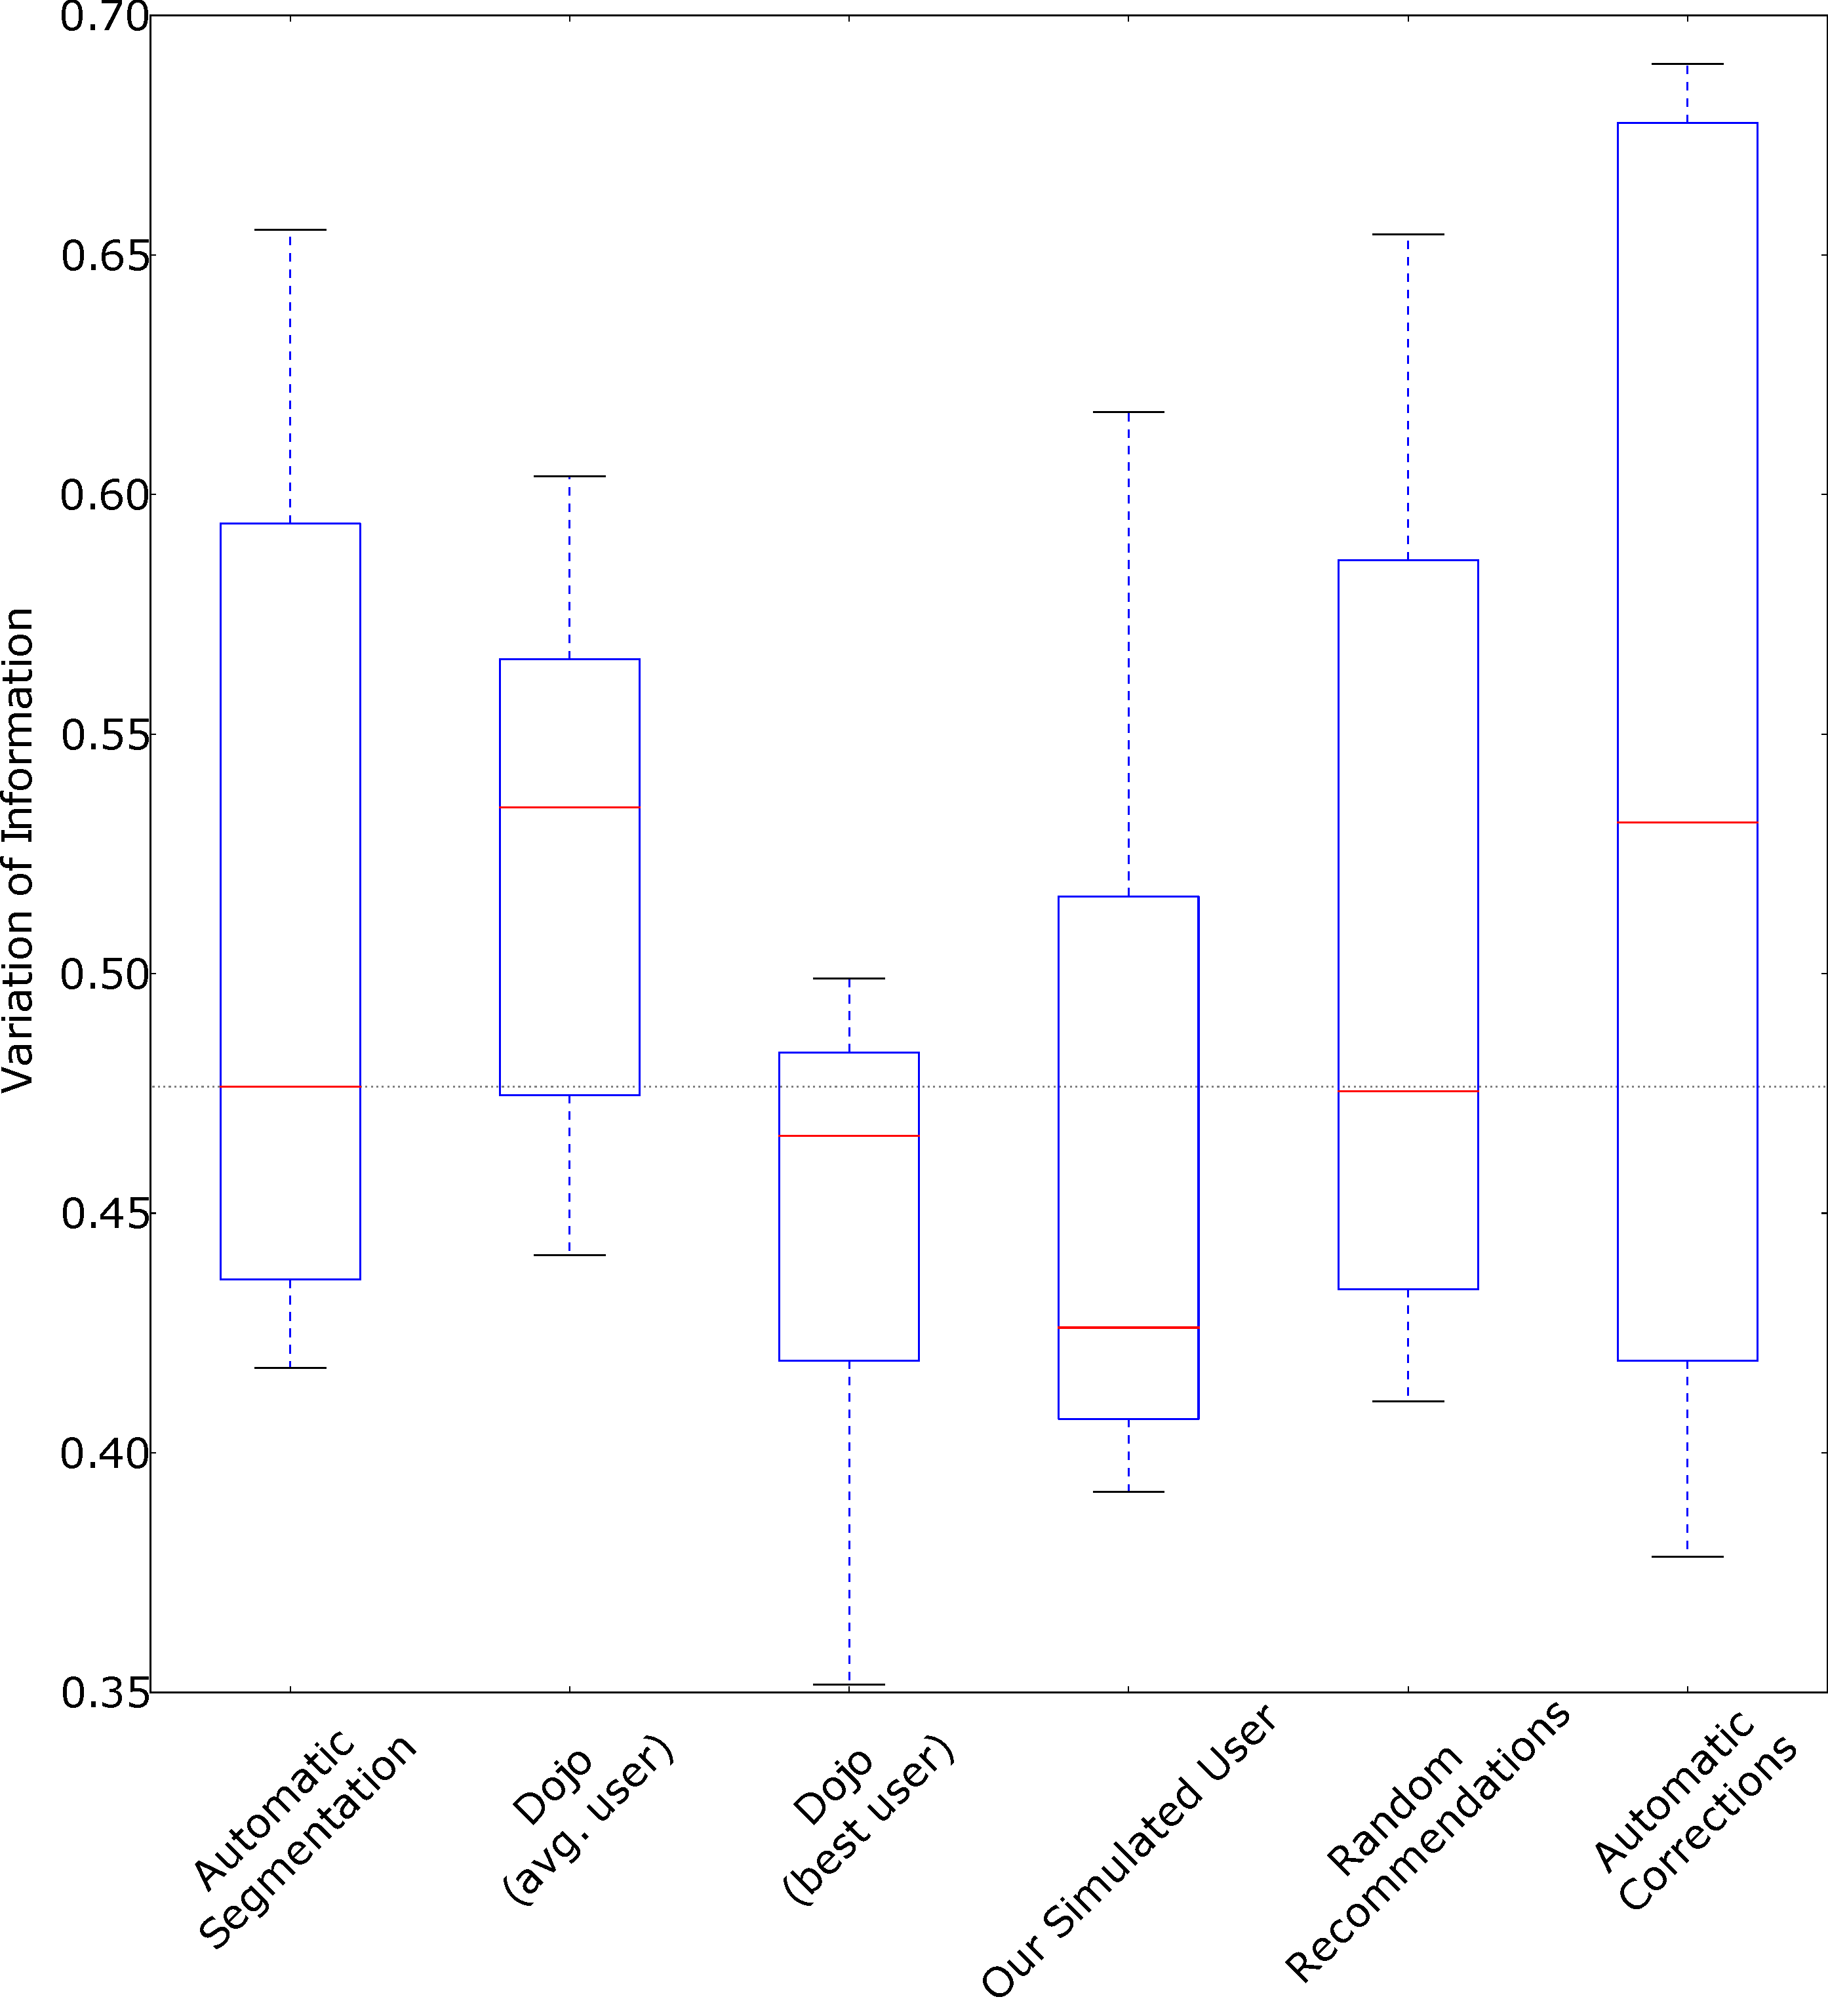
\includegraphics[scale=.2]{gfx/results_0129AM_latest.pdf}
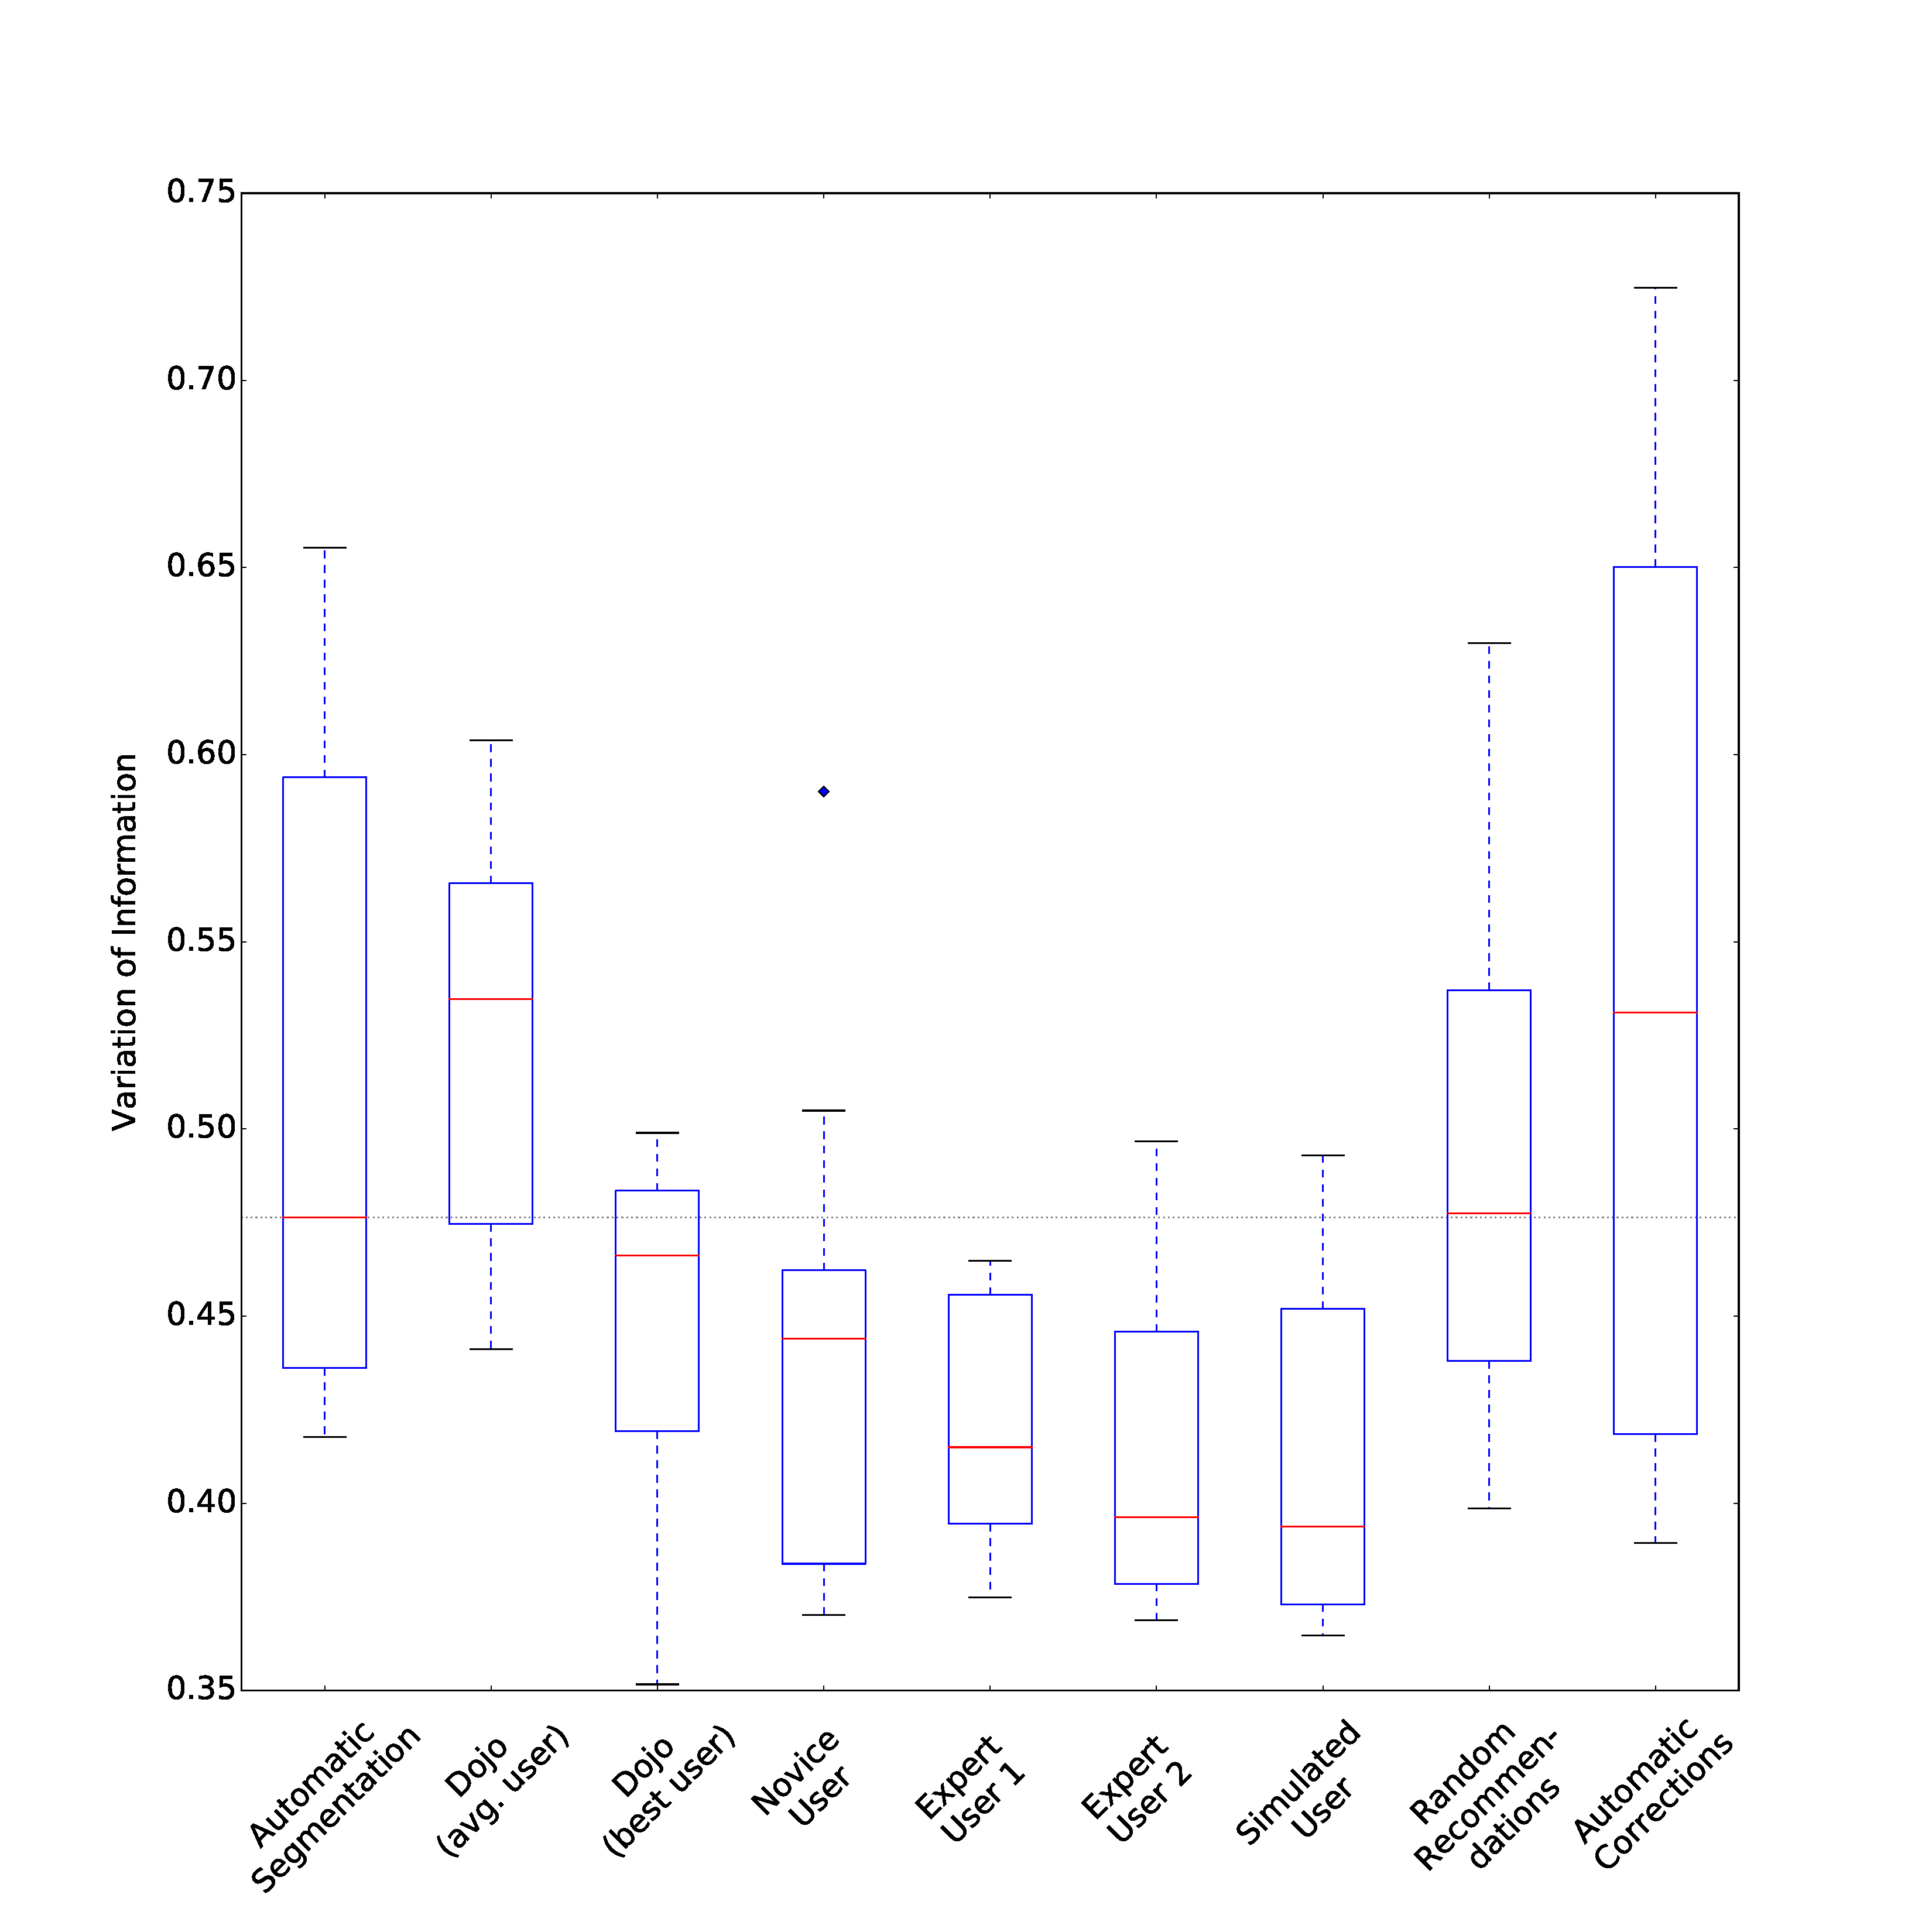
\includegraphics[scale=.2]{gfx/all_users_vi_dojo.pdf}
%	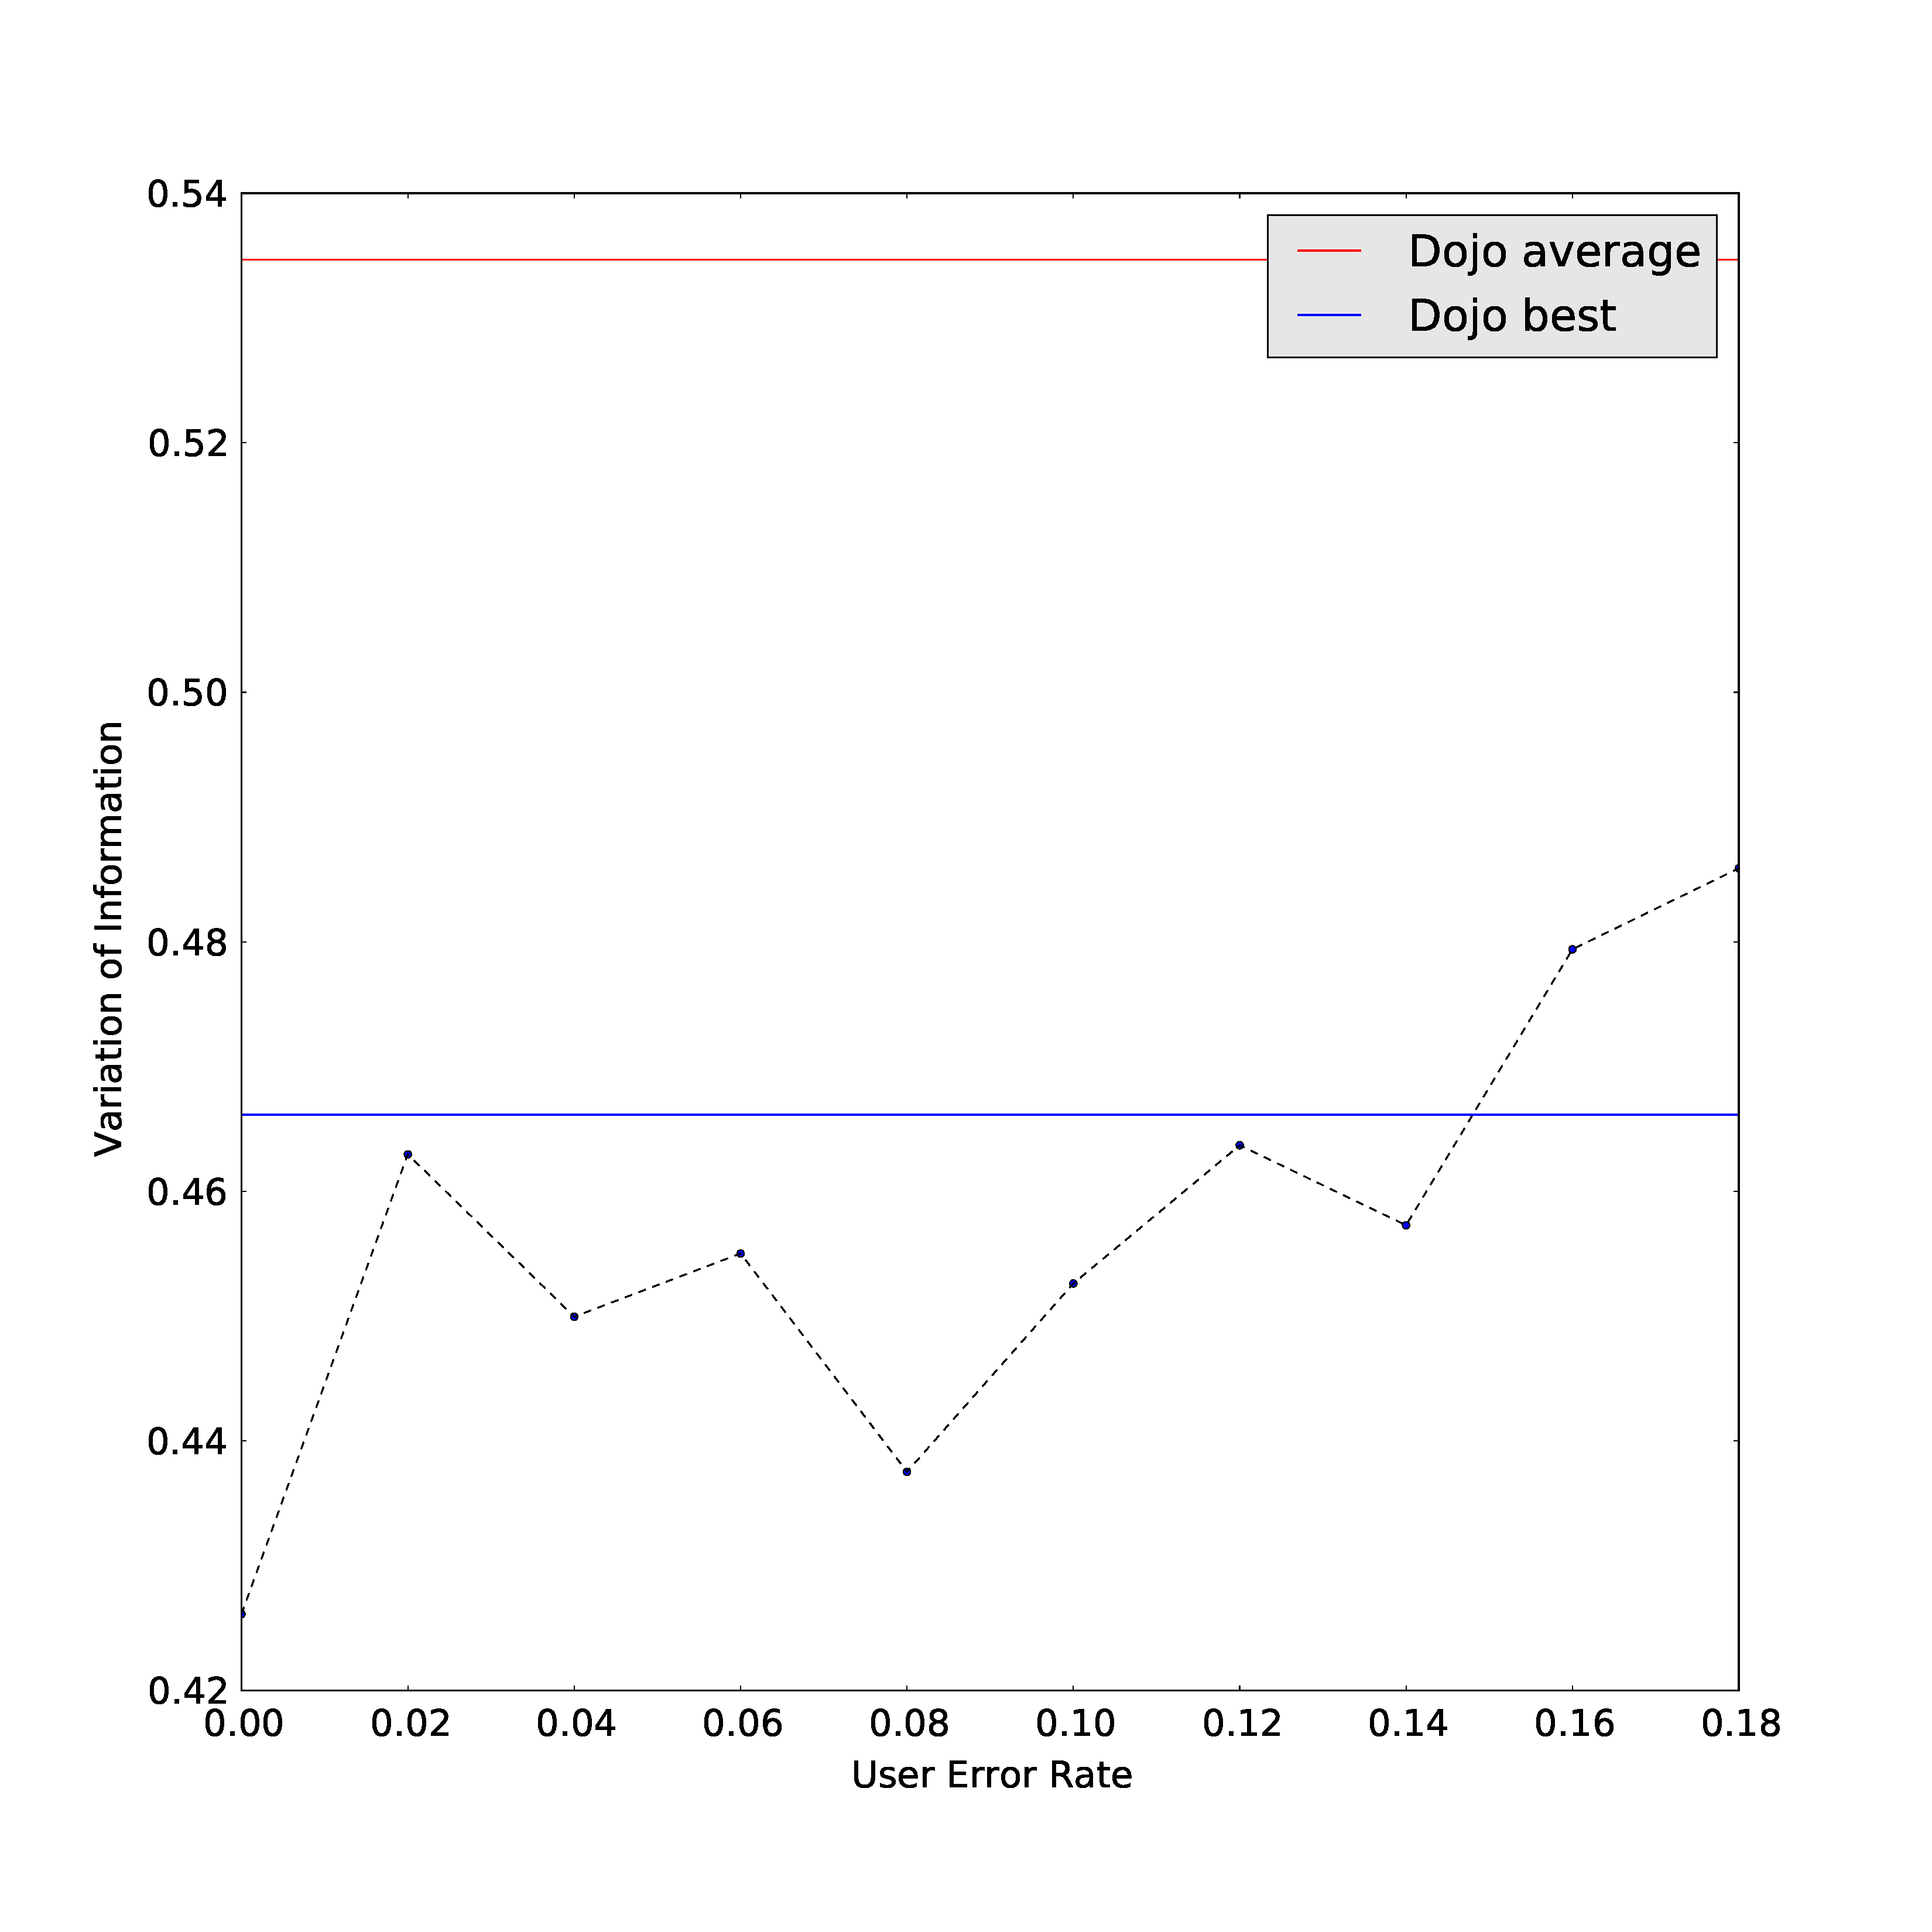
\includegraphics[scale=.10]{gfx/new_er.pdf}
	%}
	%\subfloat[Simulated user VI vs. user error rate\label{fig:simusererrorrate}]{%
	%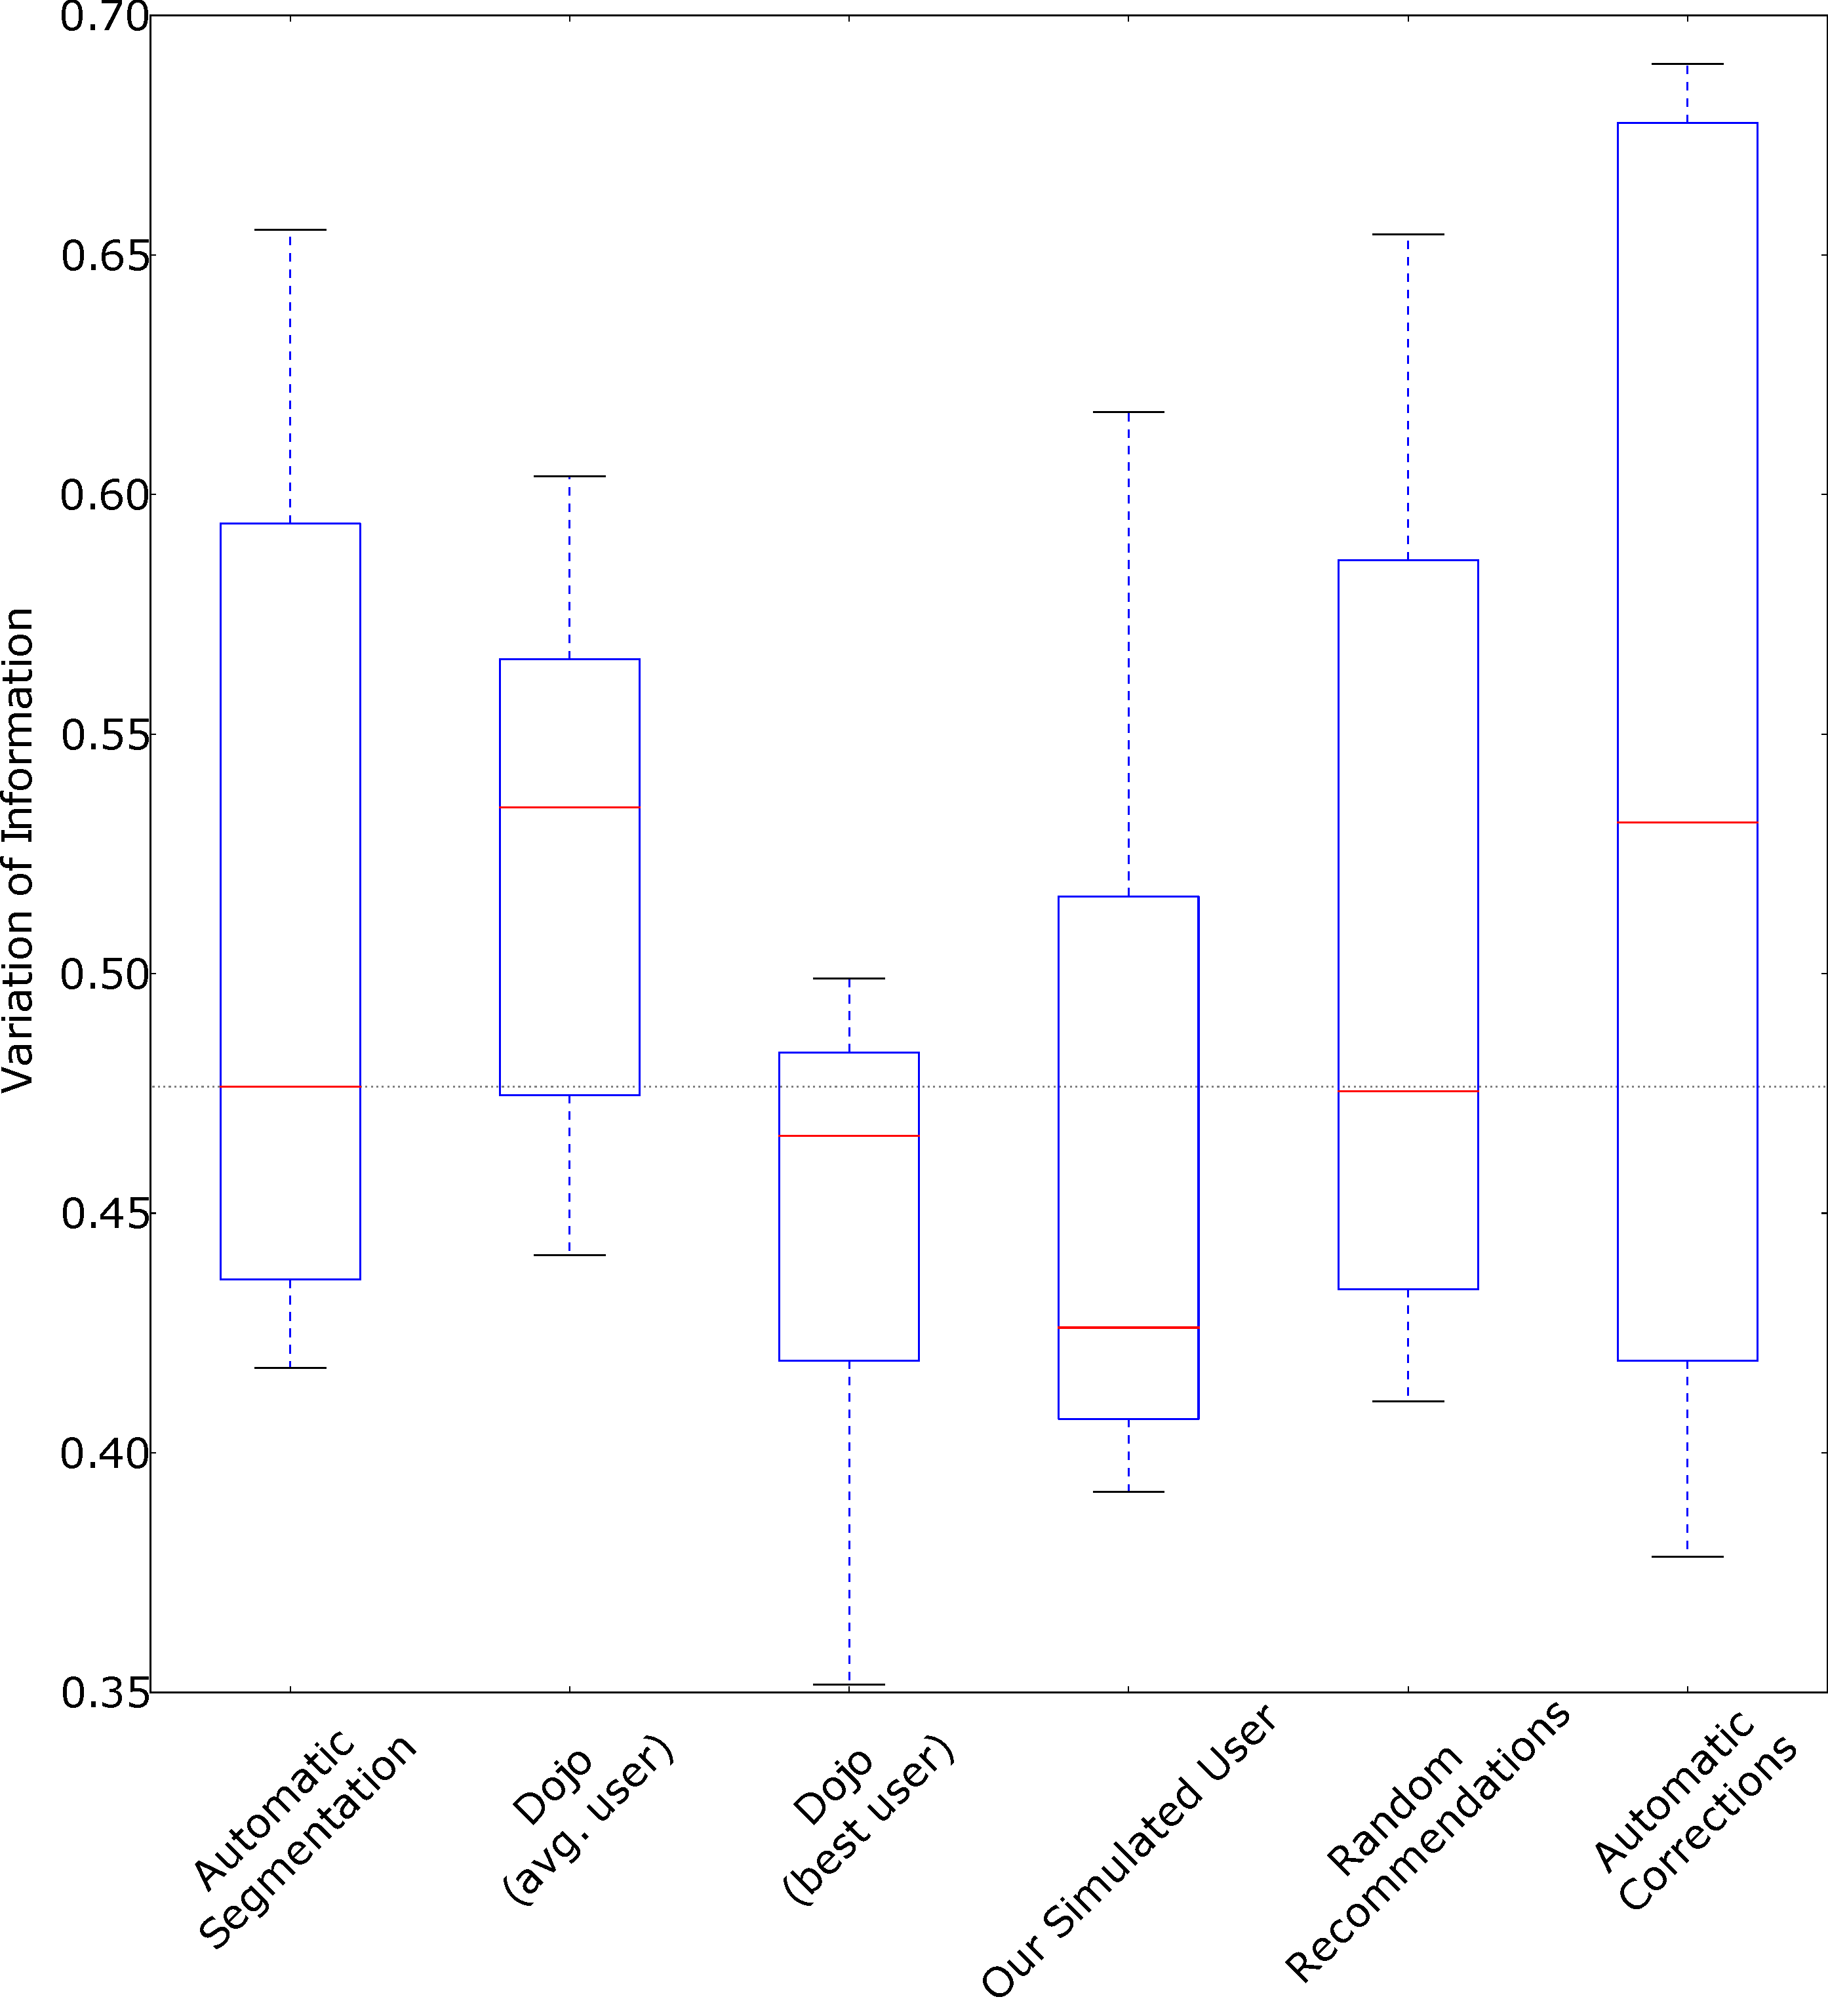
\includegraphics[scale=.08]{gfx/results_0129AM_latest.pdf}
	%}
%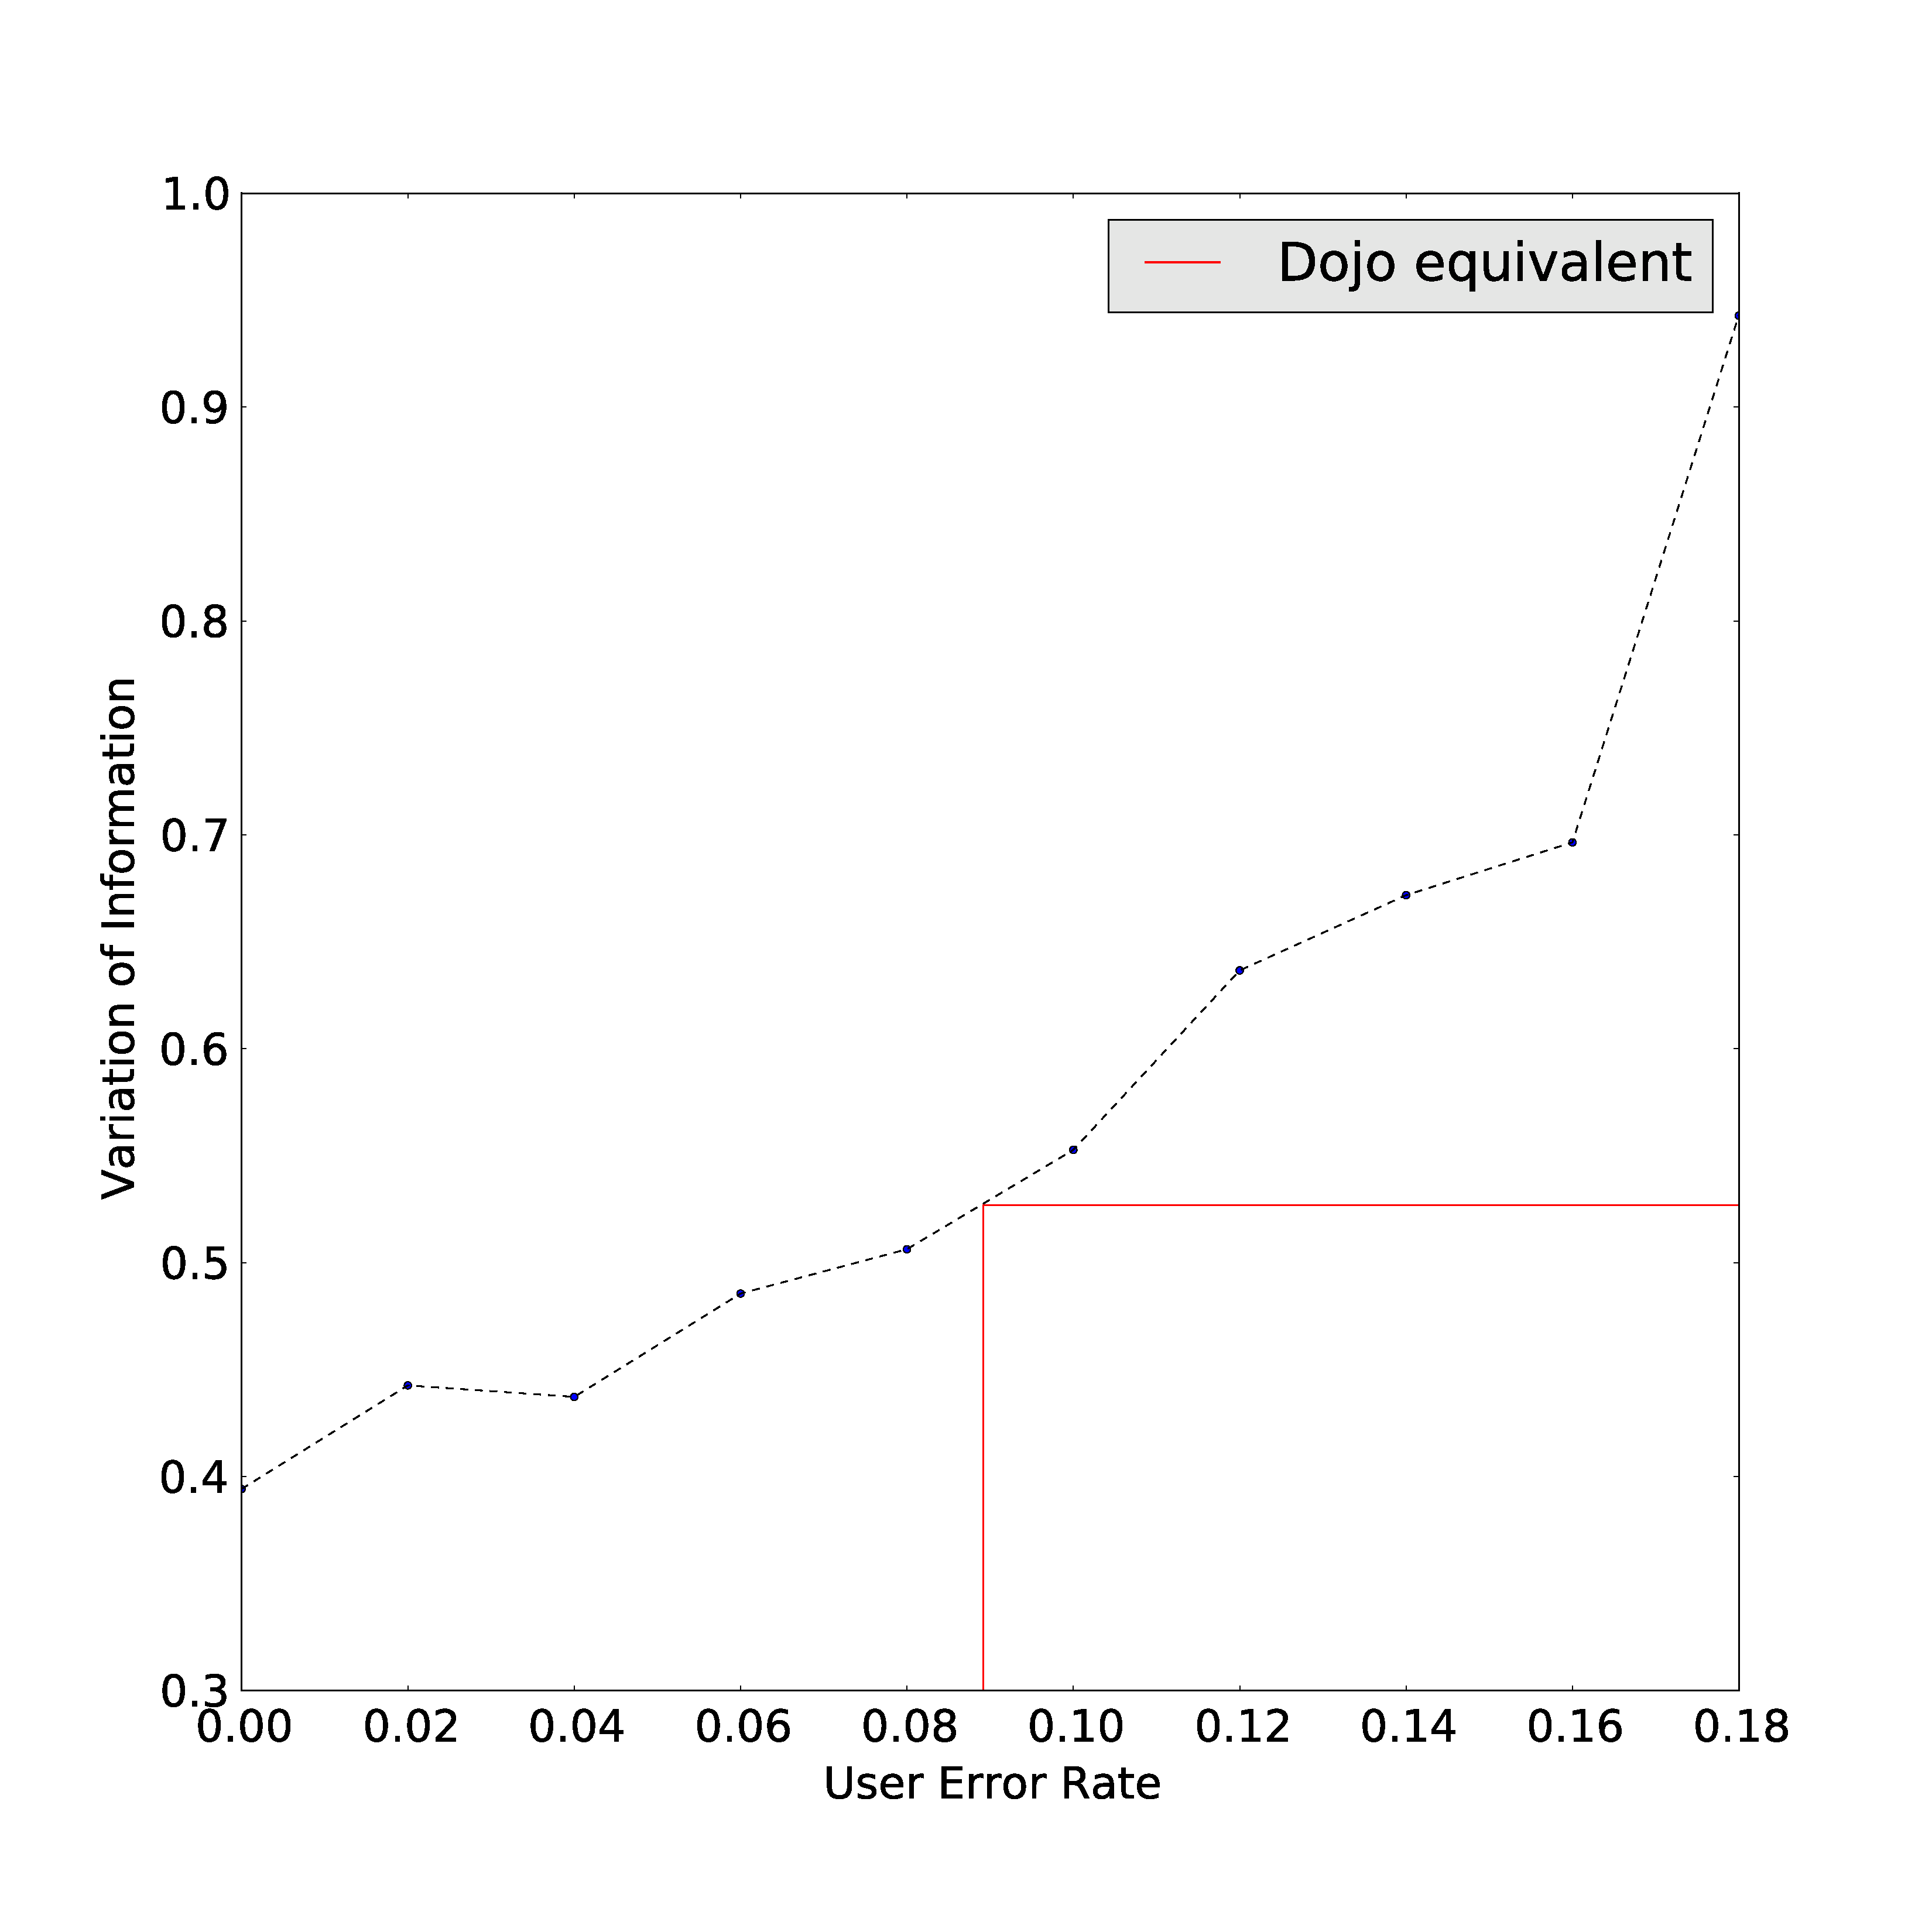
\includegraphics[scale=.1]{gfx/user_error_rate.pdf}
\caption{(a) We compare distributions of VI measures across 10 sections for the initial automatic segmentation, the average and best users in the Haehn et al.~experiment with Dojo, a novice and two experts using our system, our simulated user, our simulated user when presented with random recommendations, and finally a fully-automatic correction of recommended errors based on a threshold of acceptance. Lower scores are better.}
\label{fig:results}
\vspace{-0.4cm}
\end{figure}

\paragraph{Interactive proofreading.}
Recently, Haehn et al.~discussed requirements for interactive proofreading and evaluated three different tools on connectomics data in a study with naive users~\cite{haehn_dojo_2014}. This study asked users to spend 30 minutes proofreading with the different tools, to correct split and merge errors to improve the automatic segmentation. The best performing tool in their evaluation was Dojo. We use their findings and their user-generated proofreading result data, which they kindly provided, as a baseline for the evaluation of our method.
%The authors performed a non-expert user study and stated that their software Dojo provides better results than other tools due to a minimalistic user interface and sophisticated 3D volume rendering.
Haehn et al. perform their user study on the most representative sub-volume ($400\times400\times10$ voxels) in terms of distribution of object size. For optimal comparison, we use exactly the same data. We asked a novice and two experts to perform the proofreading task using our system (Fig.~\ref{fig:prototype}).

In addition, we simulate a user for proofreading correction. We assume that all classification has been computed ahead of time, and that the user is presented with a stream of error corrections to assess. The assessment is simulated by comparing the VI before and after each performed correction. Corrections are accepted only when VI reduces, and we test this across different user error rates (Fig.~\ref{fig:results}). In Haehn et al., the proofreading time was limited to 30 minutes, and human participants performed 59 corrections on average ($\approx30$ seconds per correction). In our scenario, users do not need to visually find errors and manually correct them, and so instead we assume each correction assessment takes 15 seconds (120 assessments in 30 minutes). Split errors are likely to take 

\begin{wrapfigure}{r}{0.5\textwidth}
  \vspace{-0.95cm}
  \begin{center}
    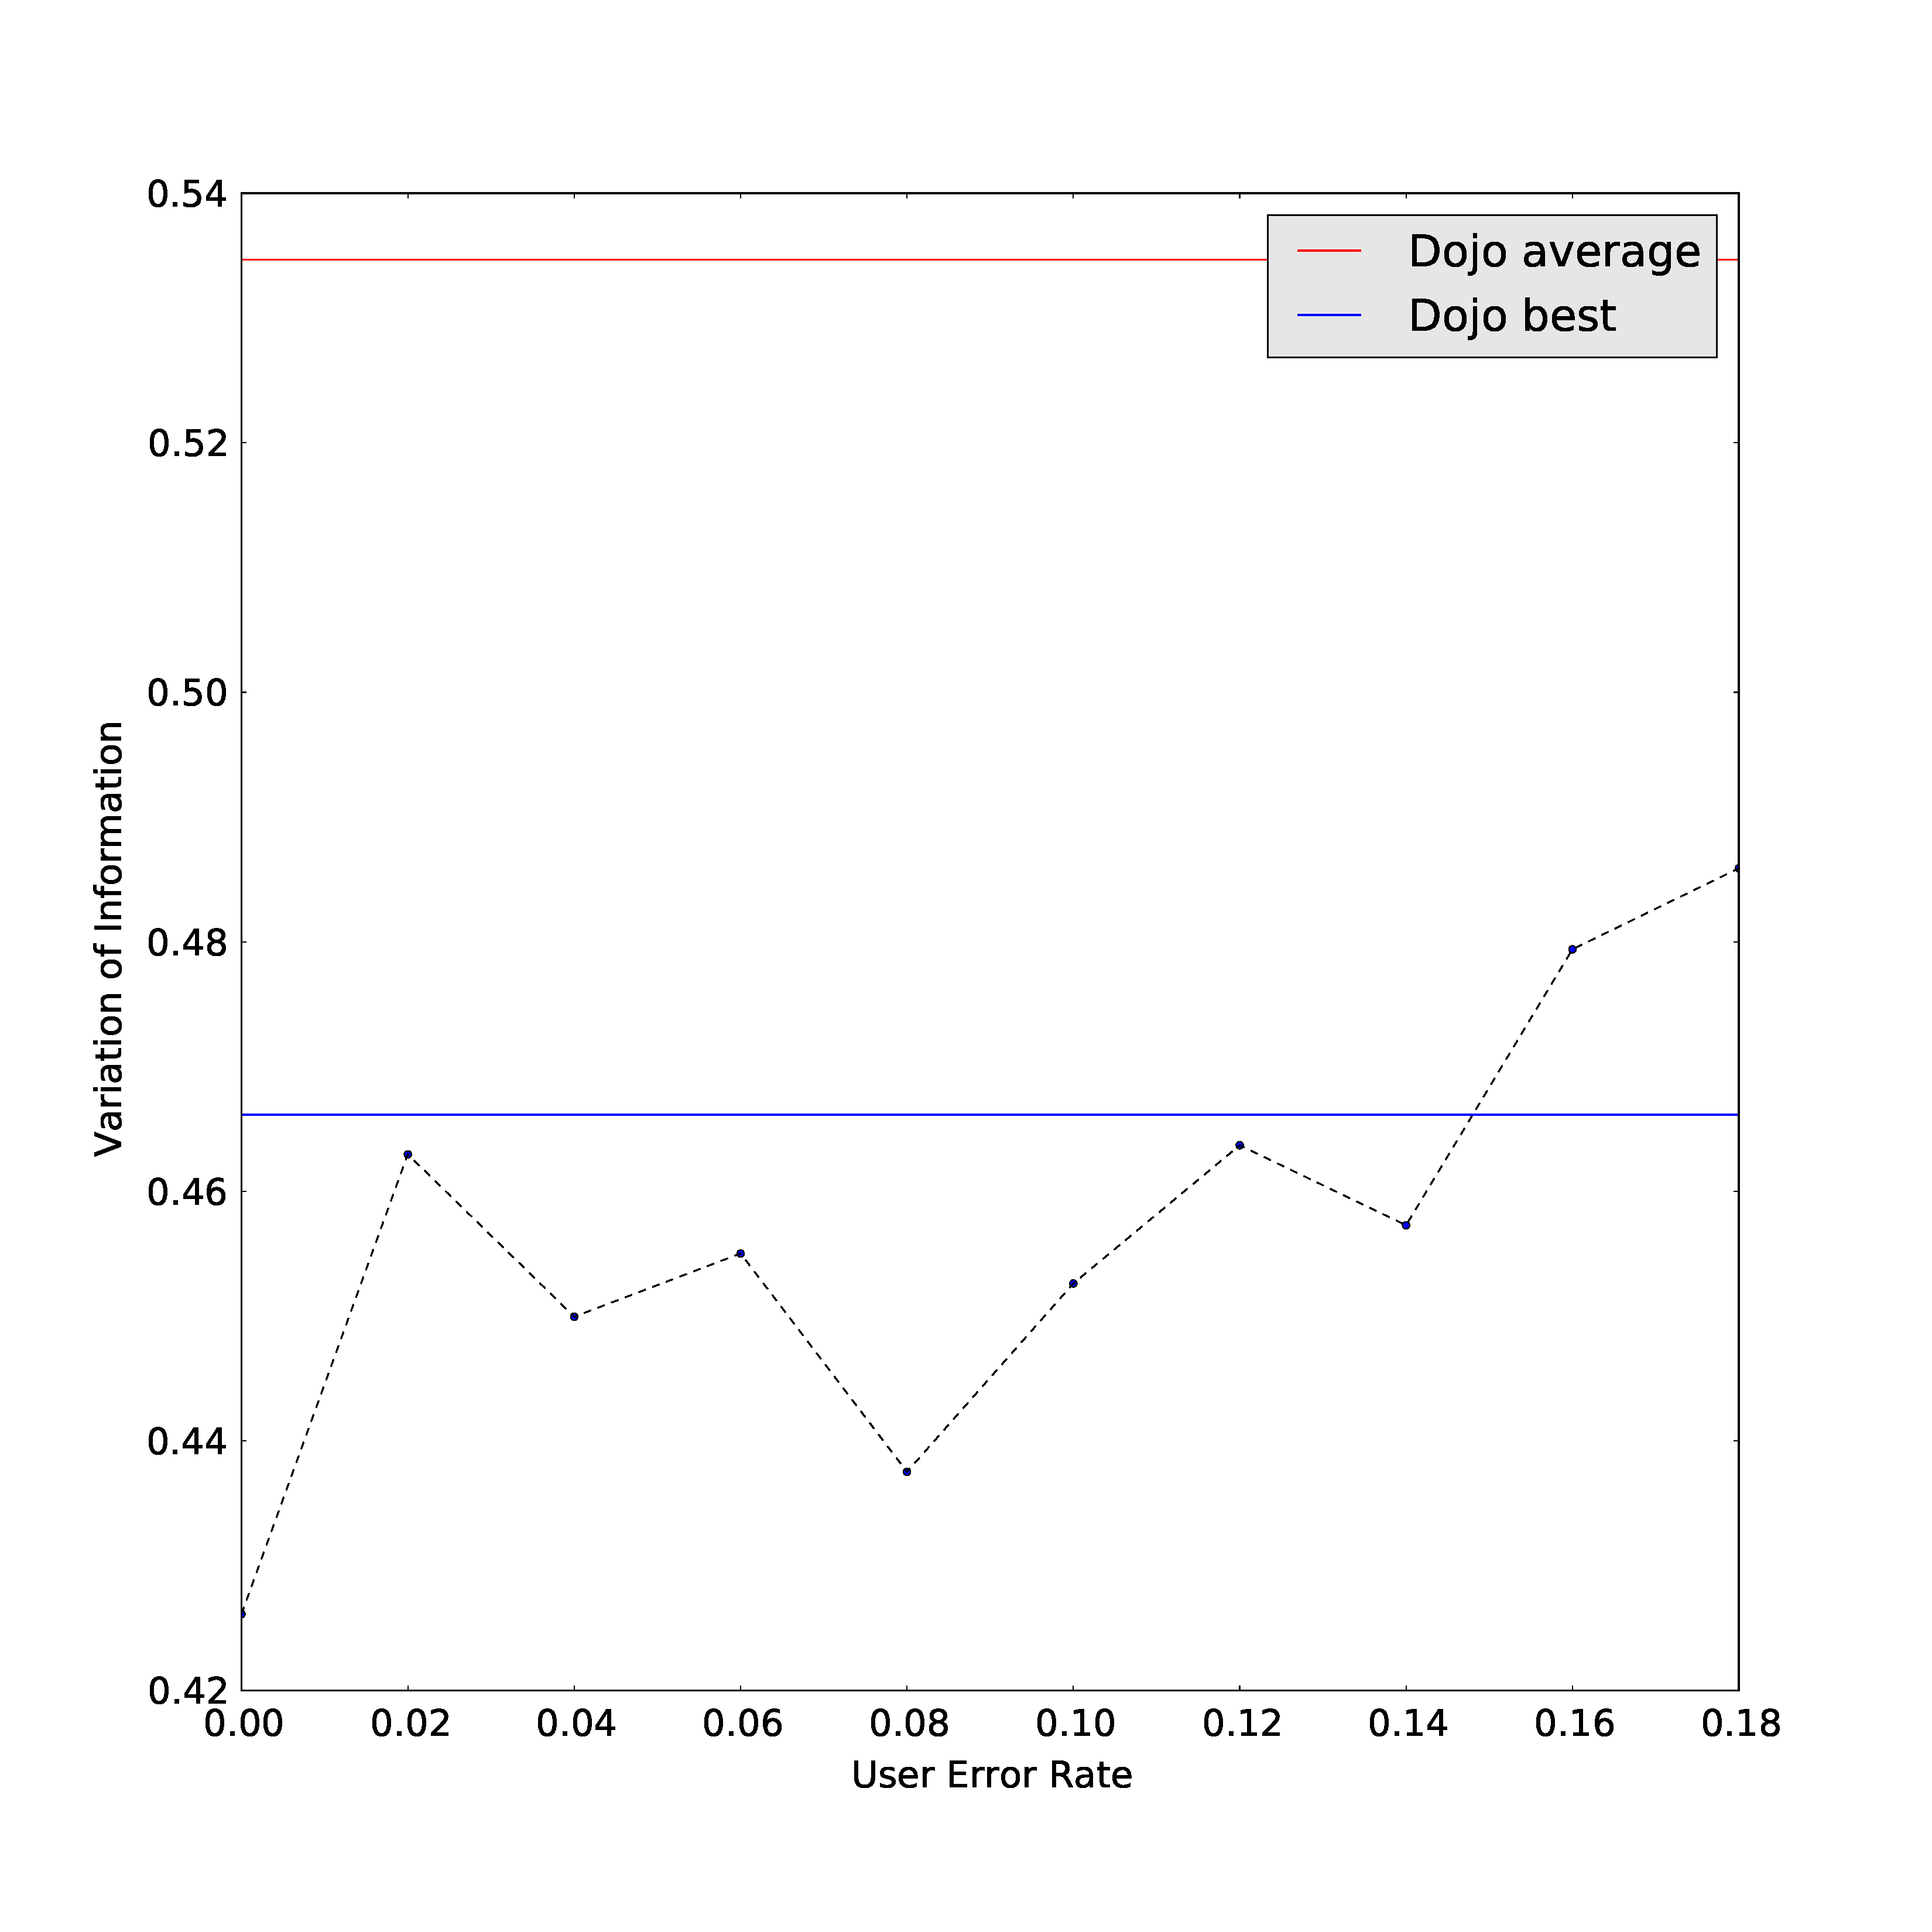
\includegraphics[scale=.1]{gfx/new_er.pdf}
  \end{center}
  \vspace{-1cm}
  \caption{VI vs.~sim.~user error rate.}
  \vspace{-1.5cm}
\end{wrapfigure}

\noindent less time than this; however, merge errors are harder to assess, as the user must select between the top 5 candidate boundaries. Since the performance between human participants of Haehn et al.'s user study shows large variation, we present both the best performing user (VI improvement: $0.0102$) and the average performance among all users (VI improvement: $-0.0582$) as our baseline. For our simulated user, the VI improvement is $0.0502$ (Fig.~\ref{fig:results}).

%, and we test this across different user error rates





\begin{figure}[t]
 \centering
    \subfloat[Split error\label{fig:layers}]{%
      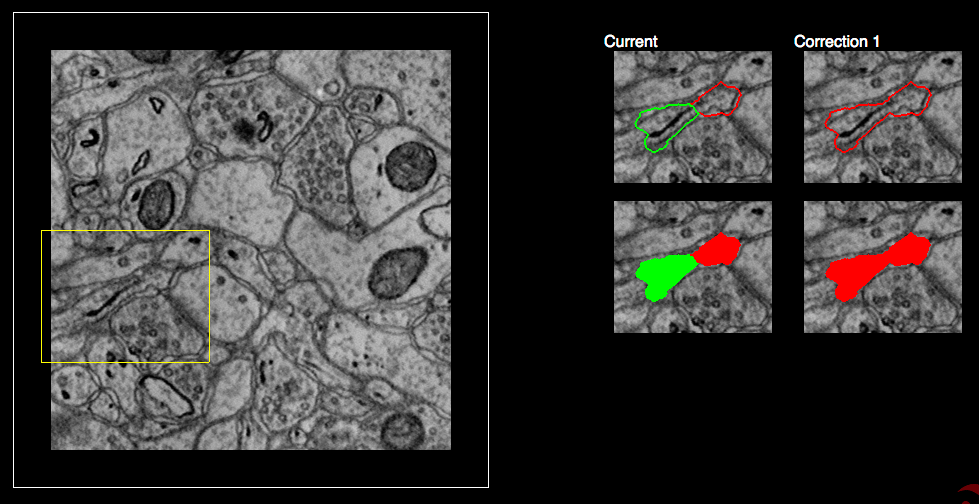
\includegraphics[width=0.47\textwidth]{gfx/proto_split.png}
    }
    \hfill
    \subfloat[Merge error\label{fig:networks}]{%
      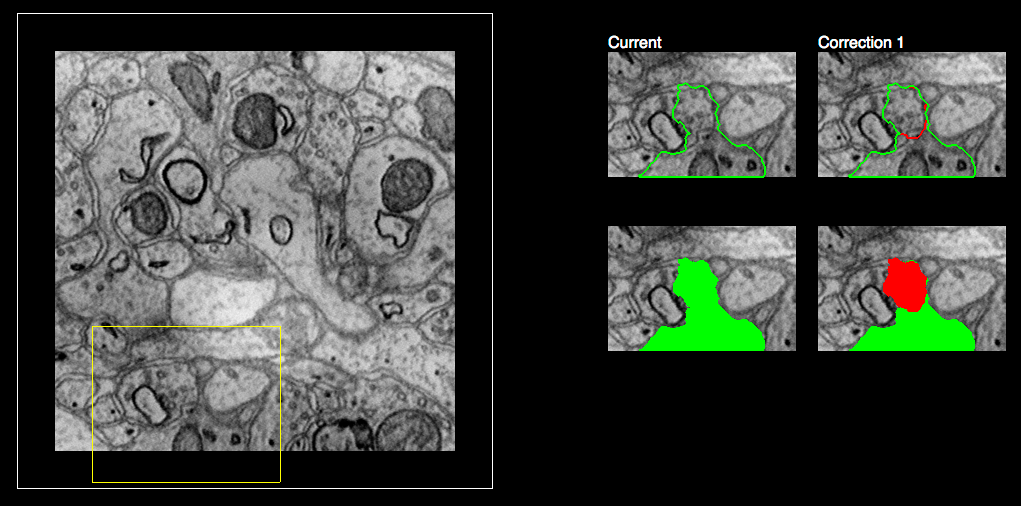
\includegraphics[width=0.49\textwidth]{gfx/proto_merge.png}
    }
	\caption{Our web-based user interface includes a slice overview with the relevant area highlighted in yellow. The interface shows (a) a split error with a suggested correction as well as (b) a merge error with correction. The user selects whether to accept a correction or to skip it.}
	\vspace{-0.4cm}
\end{figure}

\paragraph{Random recommendations.} We decided to test a classifier with random performance in comparison to our learned CNN. For split errors, the simulated user is presented with randomly picked boundaries, which they can accept or reject. For merge errors, the simulated user is presented with 5 randomly selected boundaries from the interior of the segmented region. The significantly worse performance of this approach demonstrates that our network is informative to the user.

\paragraph{Automatic correction.} As a comparison, we also perform automatic correction. During training, we define a probability threshold $p_t=0.95$ for automatic split correction based on CNN probability from the test set. Then, for automatic correction, we apply both classifiers to produce lists of split and merge errors sorted by confidence. First, we correct merge errors with $\max(1-p)$, followed by split error correction using $p_t$. The total time for correcting all errors was 17 minutes on a 3.2 GHz Quad-core Intel Xeon with an NVIDIA GeForce Titan (merge error correction 15min, split error correction 2min). The median VI improvement in comparison to the ground truth was negative, at $-0.0552$ (Fig.~\ref{fig:results}). This is not surprising, as the problem is very challenging, and this motivates the need for human-in-the-loop proofreading tools.

\begin{figure}[ht]
 \centering
    \subfloat[Split error\label{fig:layers}]{%
      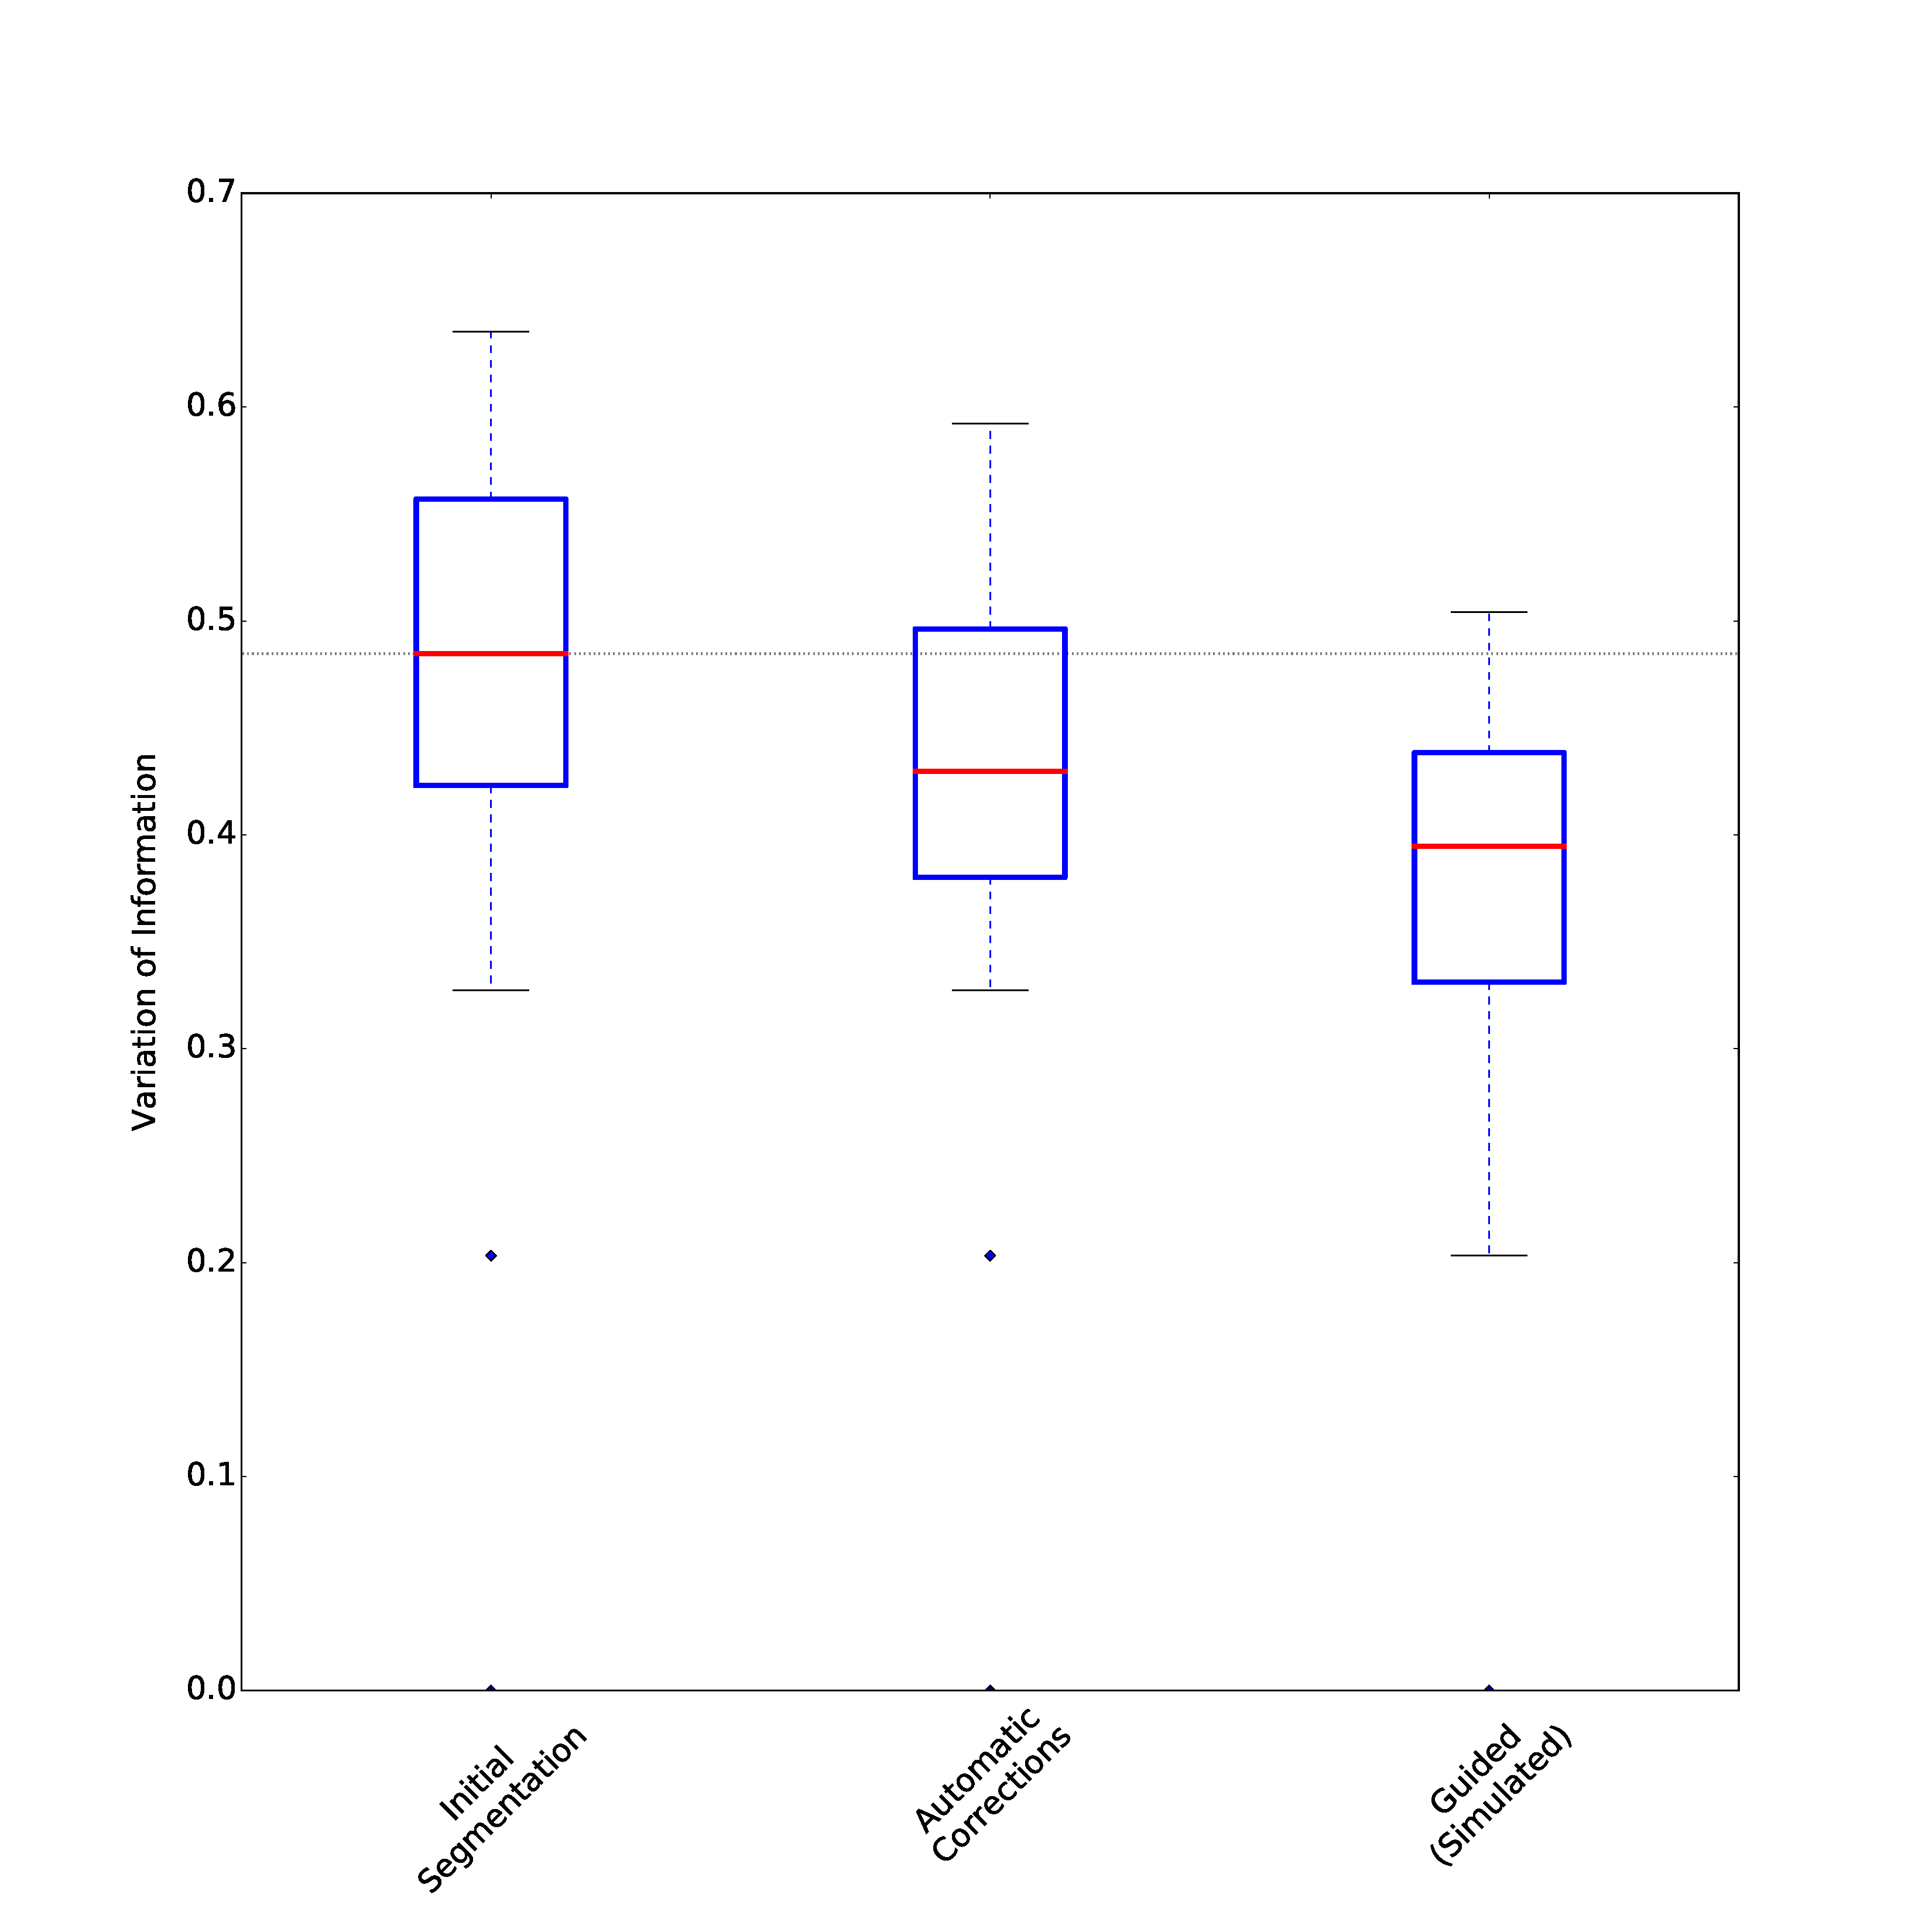
\includegraphics[width=0.49\textwidth]{gfx/cylinder_vi.pdf}
    }
    \hfill
    \subfloat[Merge error\label{fig:networks}]{%
      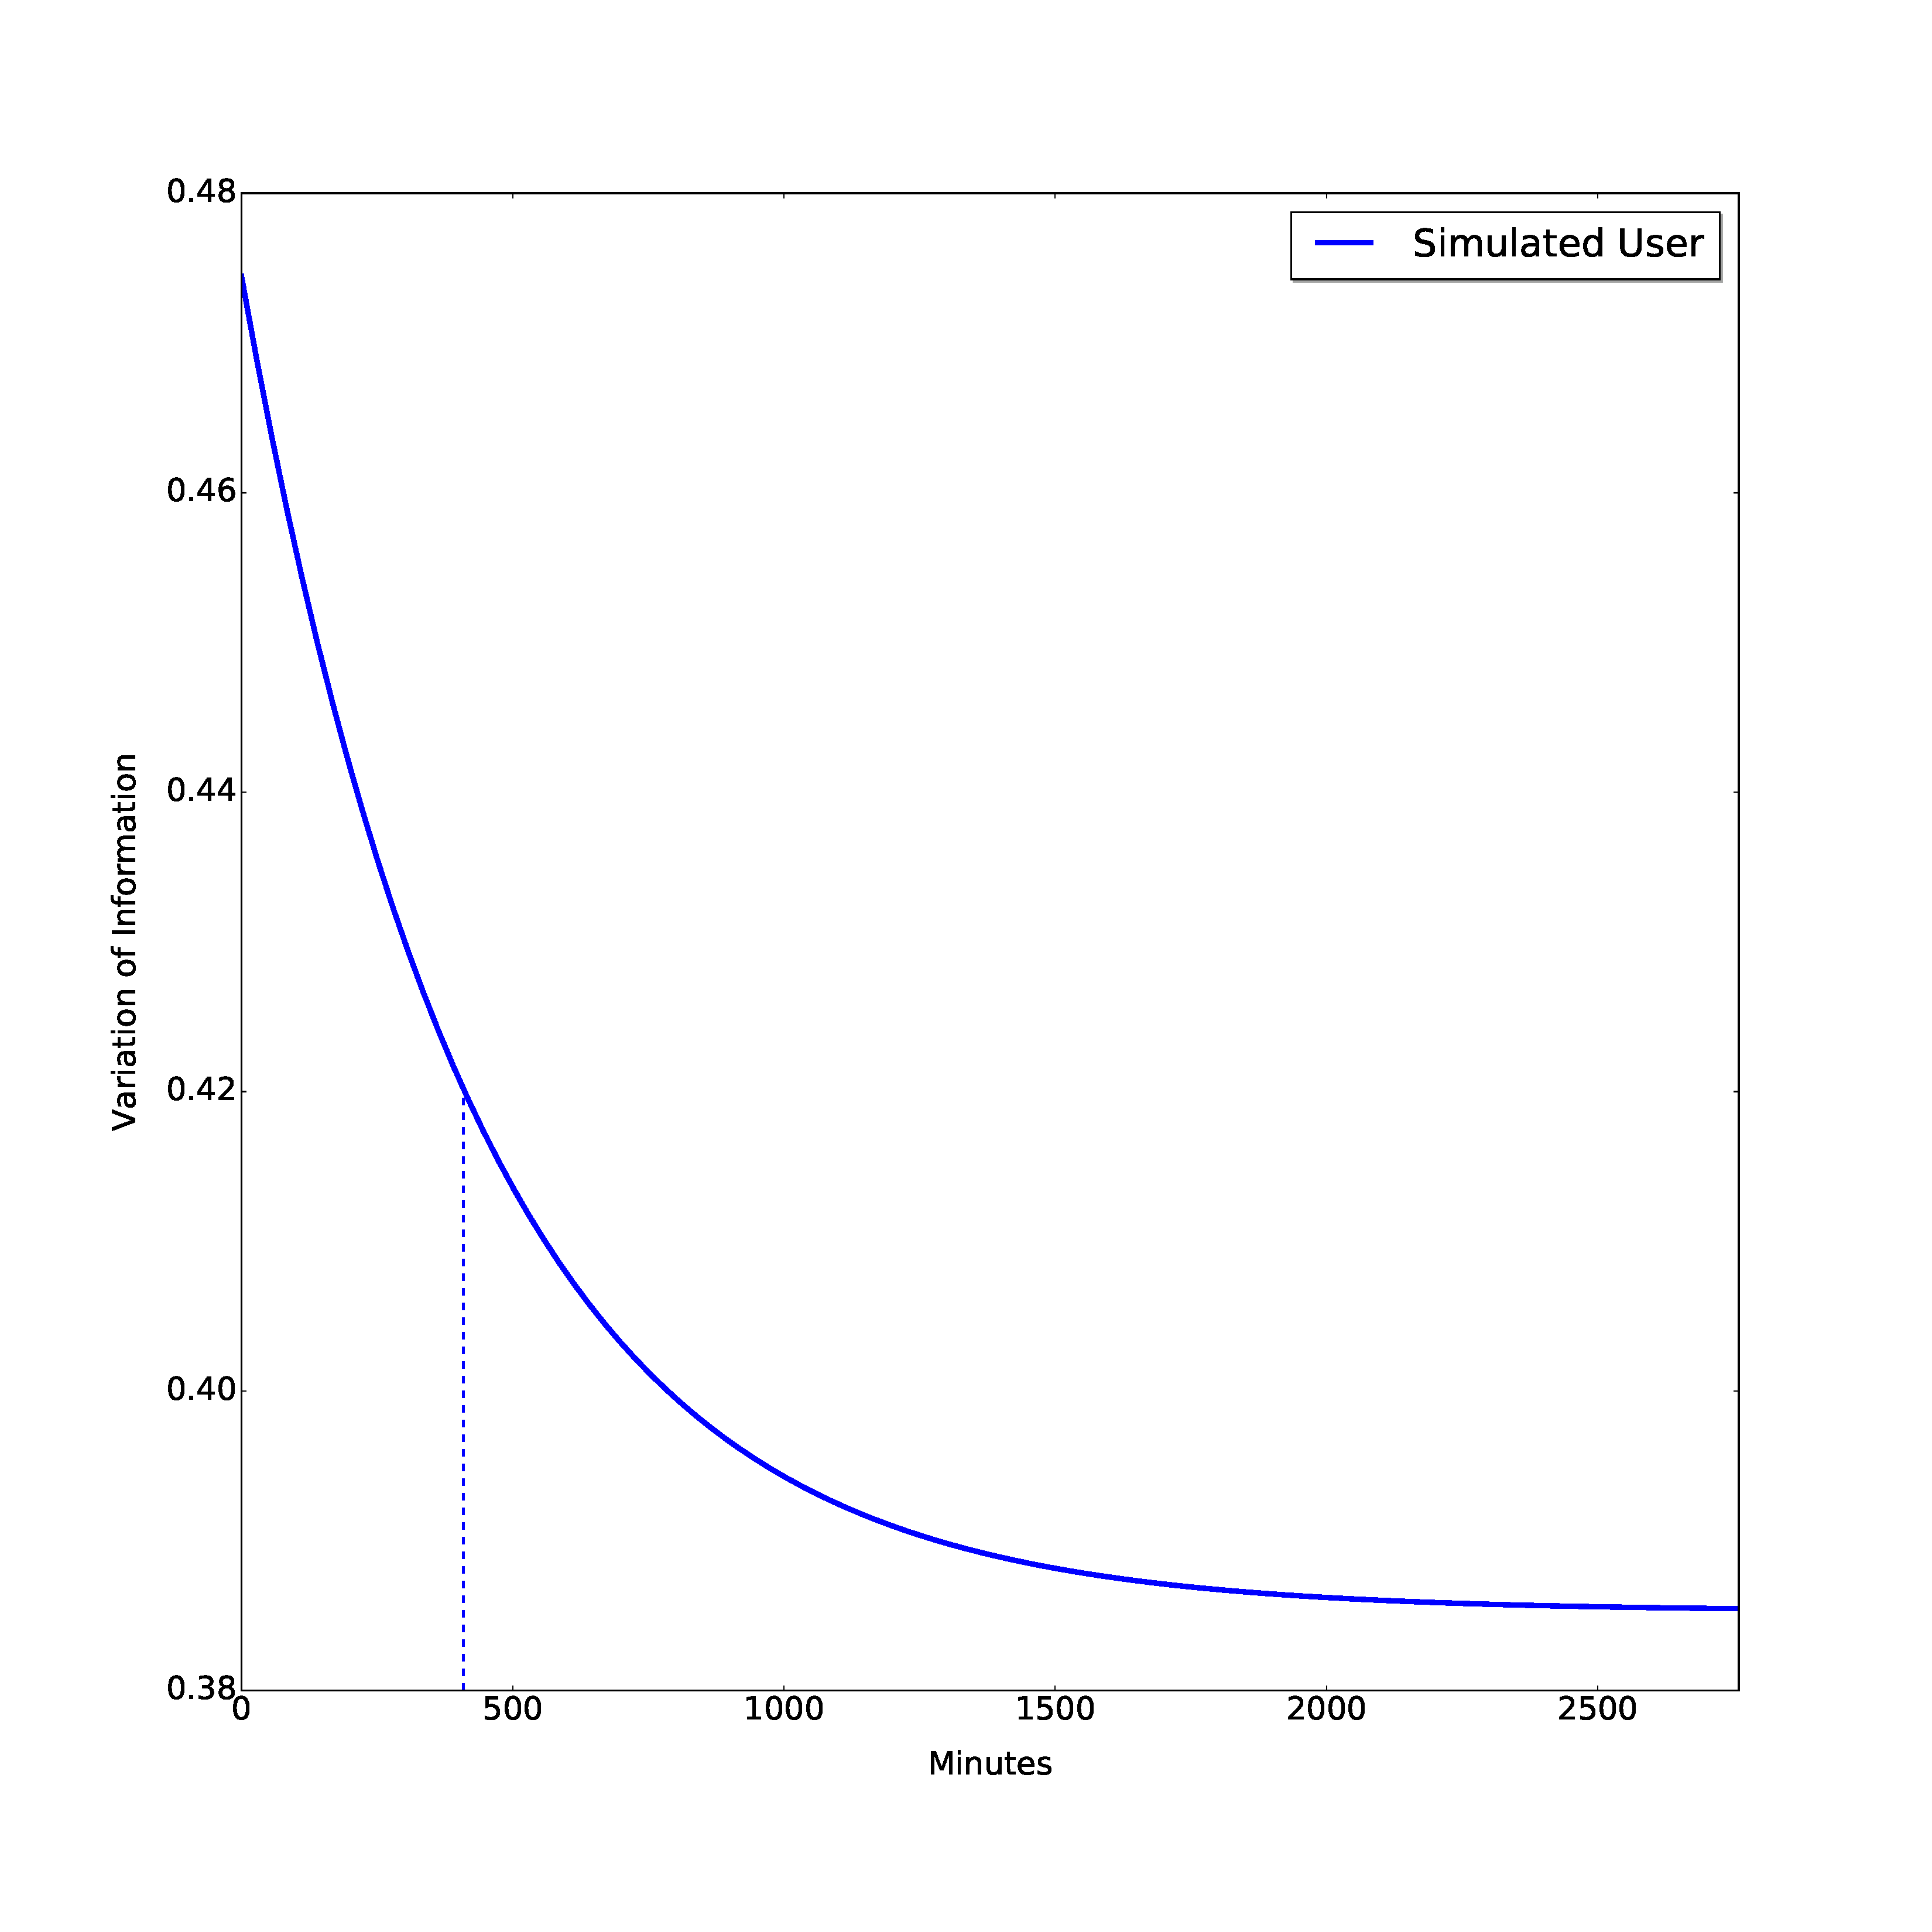
\includegraphics[width=0.49\textwidth]{gfx/simuser_vi.pdf}
    }
	\caption{Our web-based user interface includes a slice overview with the relevant area highlighted in yellow. The interface shows (a) a split error with a suggested correction as well as (b) a merge error with correction. The user selects whether to accept a correction or to skip it.}
	\vspace{-0.4cm}
\end{figure}

%
%
%\subsection{Split error evaluation}
%
%Paragraph: What is the process of evaluating split errors?
%
%Paragraph: What do we compare against? What is the result? Why is the performance better?
%
%\begin{table}[t]
%\begin{tabular}{ll}
%\toprule
%Method & VI improvement after fixing split errors \\
%\midrule
%Jain design & \\
%Jain design variation & \\
%Our design &  \\
%Our design variation & \\
%\bottomrule
%\end{tabular}
%\caption{This is a table of results. It shows the comparison to Jain et al., and the comparison to different variations of these algorithms with the varying overlap regions.}
%\label{tab:spliterrorcorrectionperformance}
%\end{table}
%
%\subsubsection{Analysis}
%
%Paragraph: Demonstration of ROC curves for VI performance in split error adjustment as the threshold varies.
%
%\begin{figure}[t]
%\missingfigure{}
%\caption{What does the performance of split error correction look like (ROC curve) as the threshold on edge probability changes?}
%\end{figure}
%
%\subsection{Merge error evaluation}
%
%Merge errors are not that common. False positive rate is very important. Choosing threshold is important.
%
%Paragraph: What is the process of evaluating merge errors?
%
%Paragraph: What do we compare against? What is the result? Why is the performance better?
%
%\begin{table}[t]
%\begin{tabular}{ll}
%\toprule
%Method & VI improvement after fixing merge errors \\
%\midrule
%Our design &  \\
%Our design variation & \\
%\bottomrule
%\end{tabular}
%\caption{This is a table of results. It shows our ability to improve VI.}
%\end{table}
%
%
%
%Philosophical point of trading split errors for merge errors...
%
%
%Speed of classification
\section{Application - Proof reading}

In our experiments, we observed the best performance using a combination of user guidance and our trained network. In contrast to fully interactive proofreading tools like Dojo, Mojo and Raveler, our system requires only minimal user input. We distinguish between merge and split errors and provide a very simple user interface to correct these (see figure \ref{fig:prototype}).
The system shows only one potential error - either a false merge or a false split - in the interface. In the case of merge errors, the user is presented the highest scoring five possible boundaries as overlays on the corresponding grayscale image and also a possibility to draw a boundary interactively. The user then chooses one of the suggestions, draws a boundary or marks the cell as correct.  For split errors, the system shows the grayscale image and a possible border and the user marks the cell as correct or indicates he wants to split. Our experiment baseline, the Dojo user study, was limited to 30 minutes and participants performed 59 corrections in average (~30 seconds per correction). Our experiments have shown that even non-experts can perform a correction using our system in 5 seconds and thus, the system increases the proofreading performance.

\section{Discussion and Conclusion}

The task of automatic cell boundary segmentation is difficult, and trying to improve such segmentations automatically as a post-process through split and error correction is, in principle, no different than trying to improve the underlying cell boundary segmentation. This is shown by the approximately equivalent VI distributions of the initial segmentation and our automatic segmentation correction (Fig.~\ref{fig:results}). Due to the task difficulty, manual proofreading of connectomics segmentations is necessary, but it is a time consuming and error-prone task, as can be seen from the Dojo human trials: on average, participants actually made the segmentations worse. However, there is value in being able to recommend to users possible regions for correction, as the time cost of proofreading is dominated by the visual search for errors.

We have addressed this problem through training a CNN to detect ambiguous regions from labeled data---in effect, (re-)learning a confidence measure on boundaries. This allows us to recommend split and merge errors, and also to recommend their corrections, which is an improvement over existing systems which just provide semi-automatic merge error correction. Through simulating users with different error rates, we have shown that, for an equivalent 30 minutes of work, correction recommendation has the potential to reduce VI over existing proofreading tools. This helps reduce the proofreading bottleneck to the analysis of large connectomics datasets. To encourage testing of our proposed architecture on more data, we provide the trained networks and classifier code as free and open source software at (link omitted for review).

% with different error rates

%\JT{Do the edges we correct come from areas where RhoANA is itself less confident? Have we just re-learned a confidence measure on RhoANA?}

%Currently it is a significant bottleneck in the analysis of large data sets in connectomics. In this paper we propose a combination of machine learning and minimal user guidance to perform segmentation corrections. Our results show that this combination makes it possible to enhance the performance as well as to decrease the required time to perform segmentation corrections. We would like to encourage testing of our proposed architecture on more data and provide the developed software and trained networks free and open source at (link omitted for review).%\footnote{The implementation, trained networks and supplementary material are available at \url{http://rhoana.org/cnnproofreading}}.

%Although, our system was not able to provide a reliable fully automatic proofreading solution, the interactive results are promising and we believe that our work leads us towards a fully automatic system. 


%The performances of the trained networks were limited based on the lack of ground truth data matching our automatic segmentation pipeline. For baseline comparison, we chose a recently published user study comparing interactive proofreading tools \cite{haehn_dojo_2014}. This comparison makes sense but unfortunately the used dataset is very small. Furthermore, we would like to have non-experts and experts test our proofreading application with minimal user input.




{\small
\bibliographystyle{ieee}
\bibliography{paper_references}
}

\end{document}
